\documentclass{beamer}
\usetheme{Warsaw}


\iftrue

\setbeamercolor{normal text}{fg=white,bg=black!90}
\setbeamercolor{structure}{fg=white}

\setbeamercolor{alerted text}{fg=red!85!black}

\setbeamercolor{item projected}{use=item,fg=black,bg=item.fg!35}

\setbeamercolor*{palette primary}{use=structure,fg=structure.fg}
\setbeamercolor*{palette secondary}{use=structure,fg=structure.fg!95!black}
\setbeamercolor*{palette tertiary}{use=structure,fg=structure.fg!90!black}
\setbeamercolor*{palette quaternary}{use=structure,fg=structure.fg!95!black,bg=black!80}

\setbeamercolor*{framesubtitle}{fg=white}

\setbeamercolor*{block title}{parent=structure,bg=black!60}
\setbeamercolor*{block body}{fg=black,bg=black!10}
\setbeamercolor*{block title alerted}{parent=alerted text,bg=black!15}
\setbeamercolor*{block title example}{parent=example text,bg=black!15}

\fi


\begin{document}

{
    \usebackgroundtemplate
    {
        \vbox to \paperheight{\vfil\hbox to \paperwidth{\hfil

        {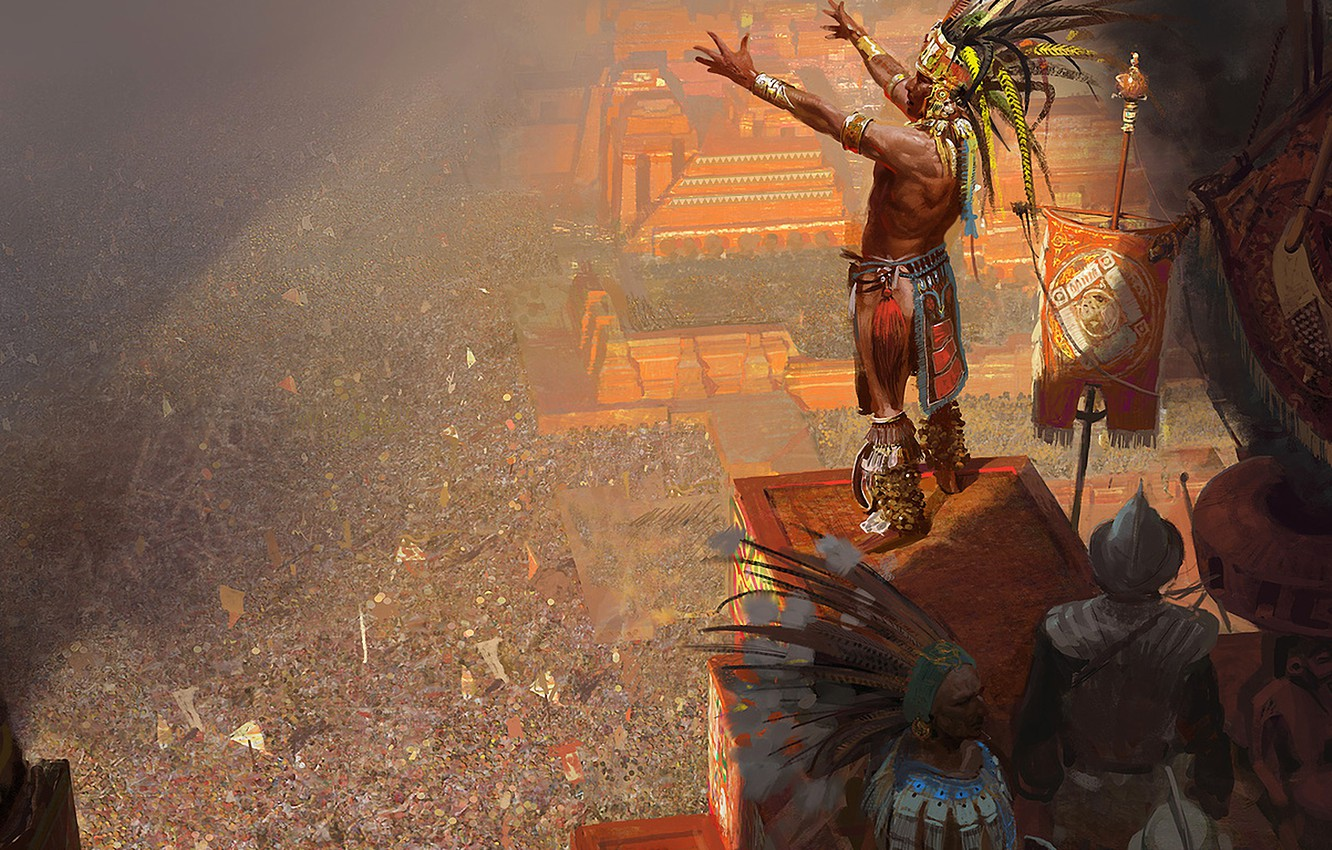
\includegraphics[width=5.05in]{../images/aztec.jpg}}

        \hfil}\vfil}
    }

    \begin{frame}
     \centering
     {
        \begin{minipage}{10cm}
           {\LARGE \color{white}{\bf reinforcement learning}} \\
           {\LARGE \color{white}{\bf current problems}} \\
           {\LARGE \color{white}{\bf Michal CHOVANEC, PhD.}} \\
       \end{minipage}
     }

    \end{frame}
}

\begin{frame}
\frametitle{reinforcement learning}

\begin{columns}

  \begin{column}{0.5\textwidth}
    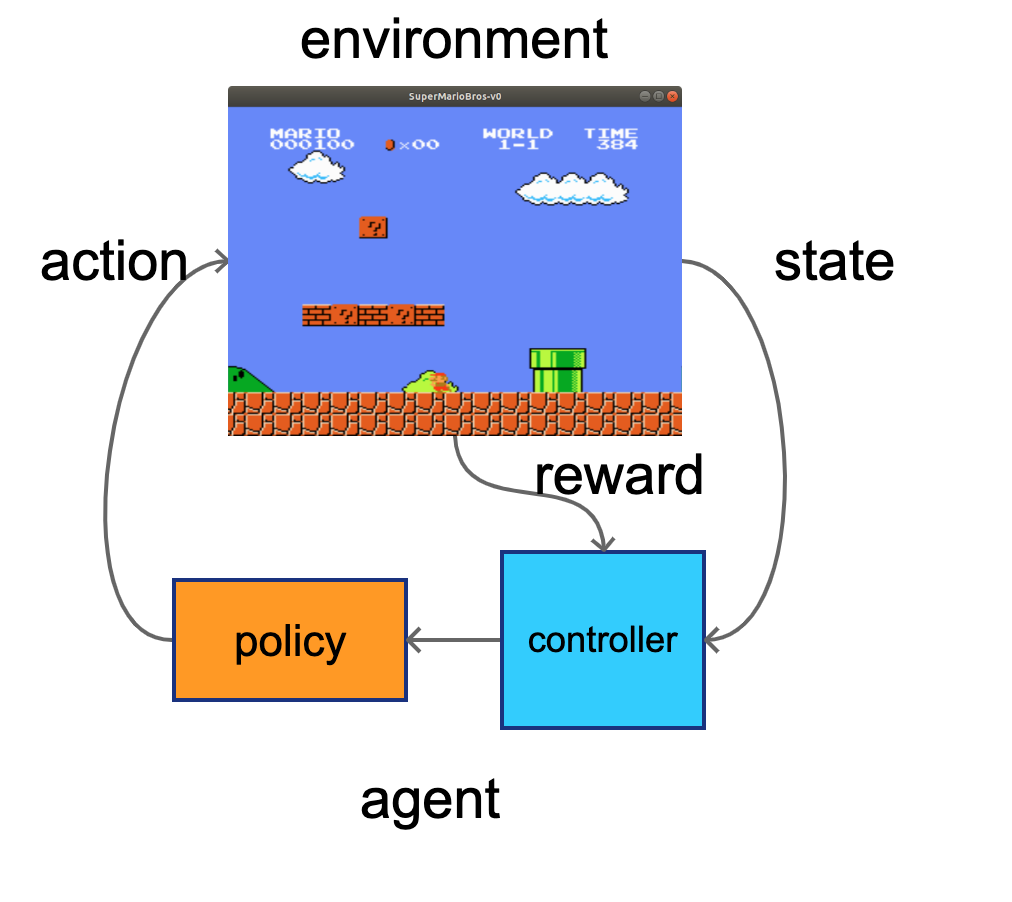
\includegraphics[scale=0.15]{../diagrams/basic/reinforcementlearning.png}
  \end{column}

  \begin{column}{0.5\textwidth}
    \begin{enumerate}
      \item {\bf obtain state} - observation
      \item {\bf choose action} - policy
      \item {\bf receive reward}
      \item {\bf learn from experiences}
    \end{enumerate}
  \end{column}

\end{columns}

\end{frame}



\begin{frame}
  
  \frametitle{when it works ?} 

  \begin{itemize}
    \item {\bf dense rewards}
    \item {\bf small state space}
    \item {\bf fully observable}
  \end{itemize}

  \begin{columns}

    \begin{column}{0.5\textwidth}
      \centering
      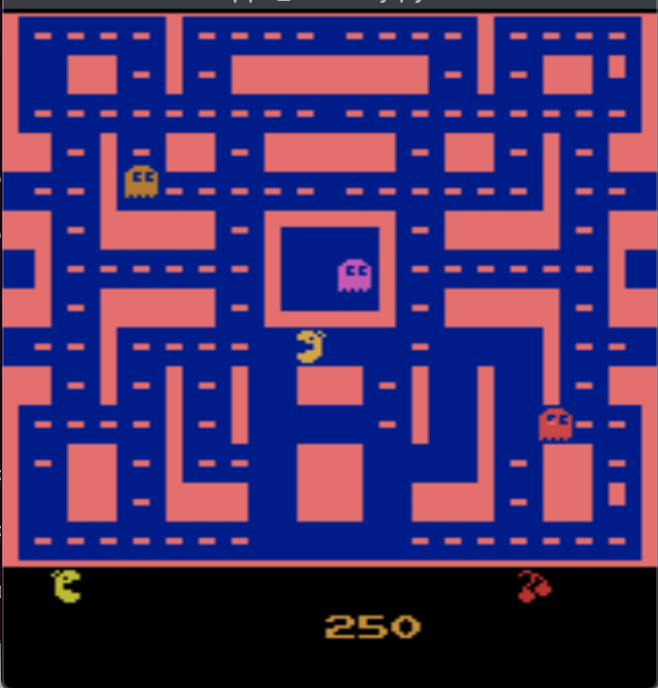
\includegraphics[scale=0.3]{../images/pacman.png}
    \end{column}

    \begin{column}{0.5\textwidth}
      \centering
      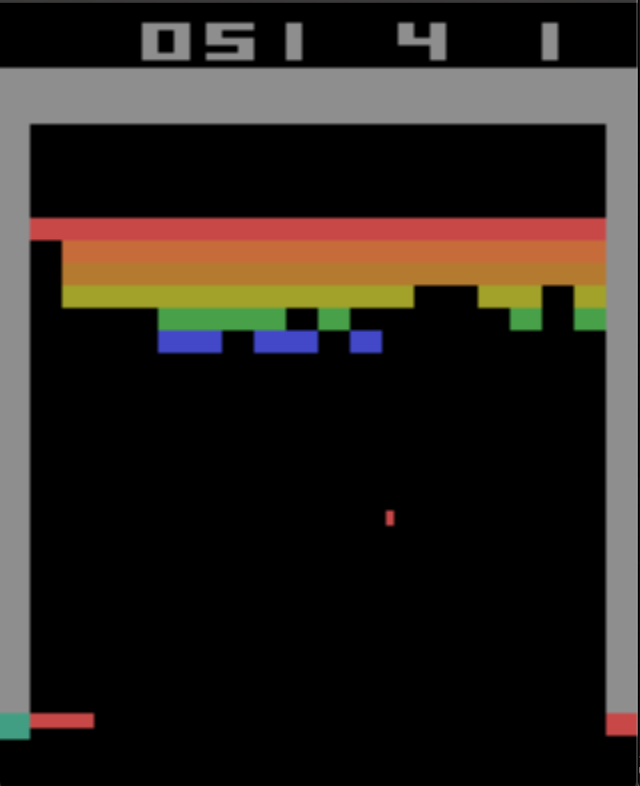
\includegraphics[scale=0.3]{../images/breakout.png}
    \end{column}
  
  \end{columns}

  
\end{frame}


\begin{frame}
  
  \frametitle{when it works - AlphaGO, AlphaZero - DeepMind} 

  \begin{columns}

    \begin{column}{0.5\textwidth}
      \centering
      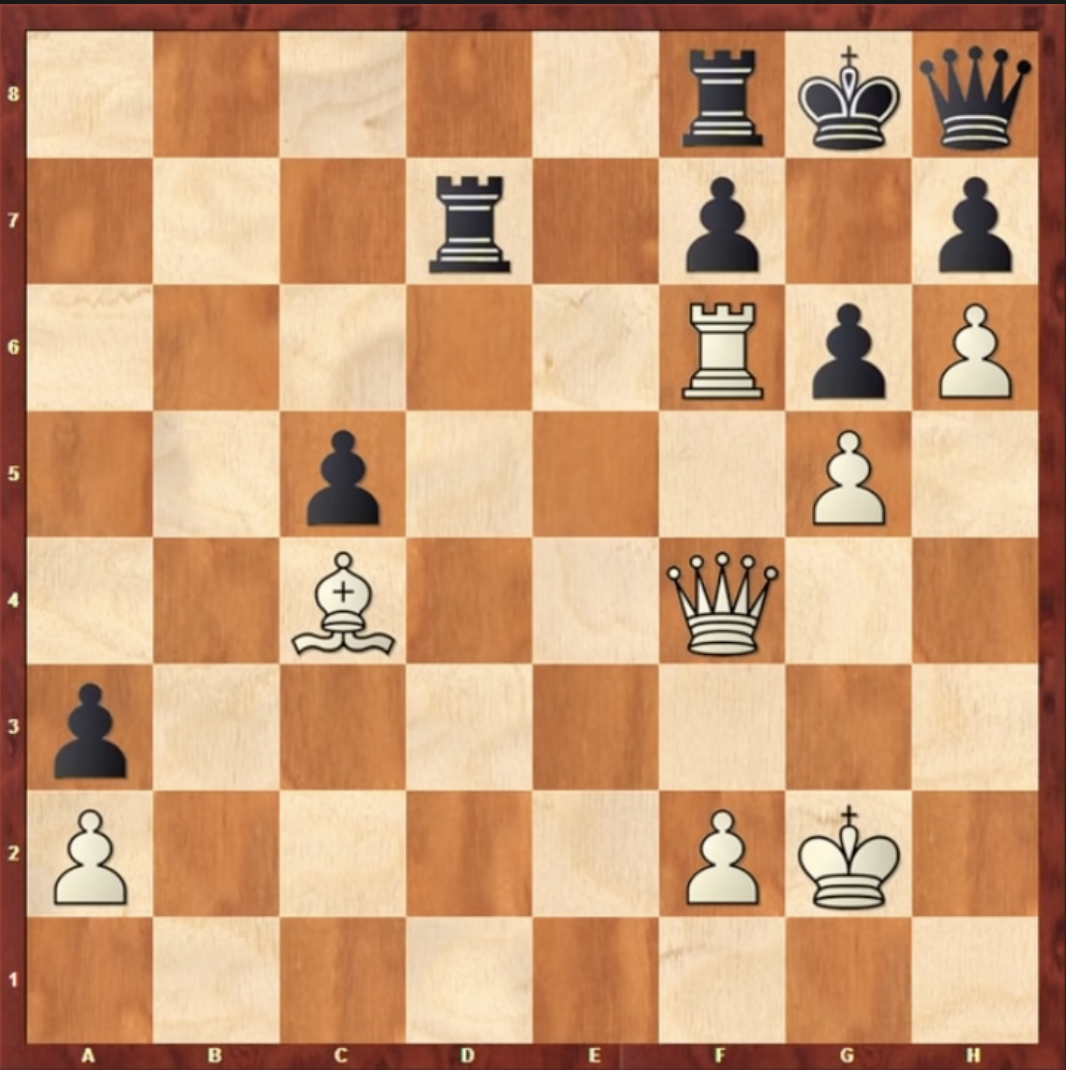
\includegraphics[scale=0.3]{../images/alpha_zero_chess.png}
    \end{column}

    \begin{column}{0.5\textwidth}
      \centering
      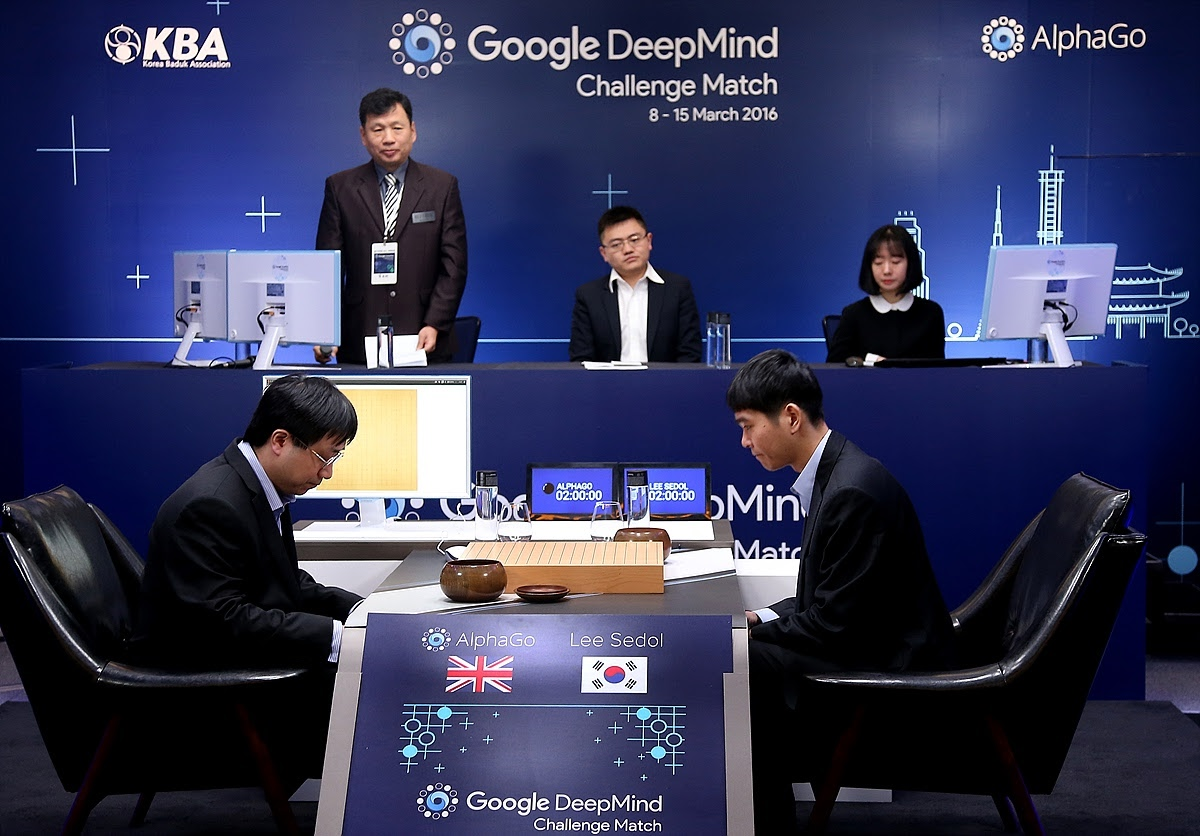
\includegraphics[scale=0.15]{../images/alpha_go.jpeg}
    \end{column}

  \end{columns}

  {\href{https://www.youtube.com/watch?v=tMab3jcTV0s}{Chess with Suren, AlphaZero's Most Astonishing "Zugzwang" Game}}

\end{frame}


\begin{frame}
  
  \frametitle{most famous algorithms} 

  \begin{itemize}
    \item deep Q network - {\bf DQN} \footnote{\href{https://arxiv.org/pdf/1312.5602.pdf}{Mnih et al. 2013}}
    \item deep deterministic policy gradient - {\bf DDPG}, D4PG \footnote{\href{https://arxiv.org/pdf/1509.02971.pdf}{Lillicrap, Hunt et al. 2016}}
    \item advantage actor critic - AC, {\bf A2C}, A3C
    \item proximal policy optimization - {\bf PPO}, TRPO \footnote{\href{https://arxiv.org/pdf/1707.06347.pdf}{Schulman, et al. 2017}}
  \end{itemize}

\end{frame}


\begin{frame}
  
  \frametitle{PPO - proximal policy optimisation} 

  \centering
  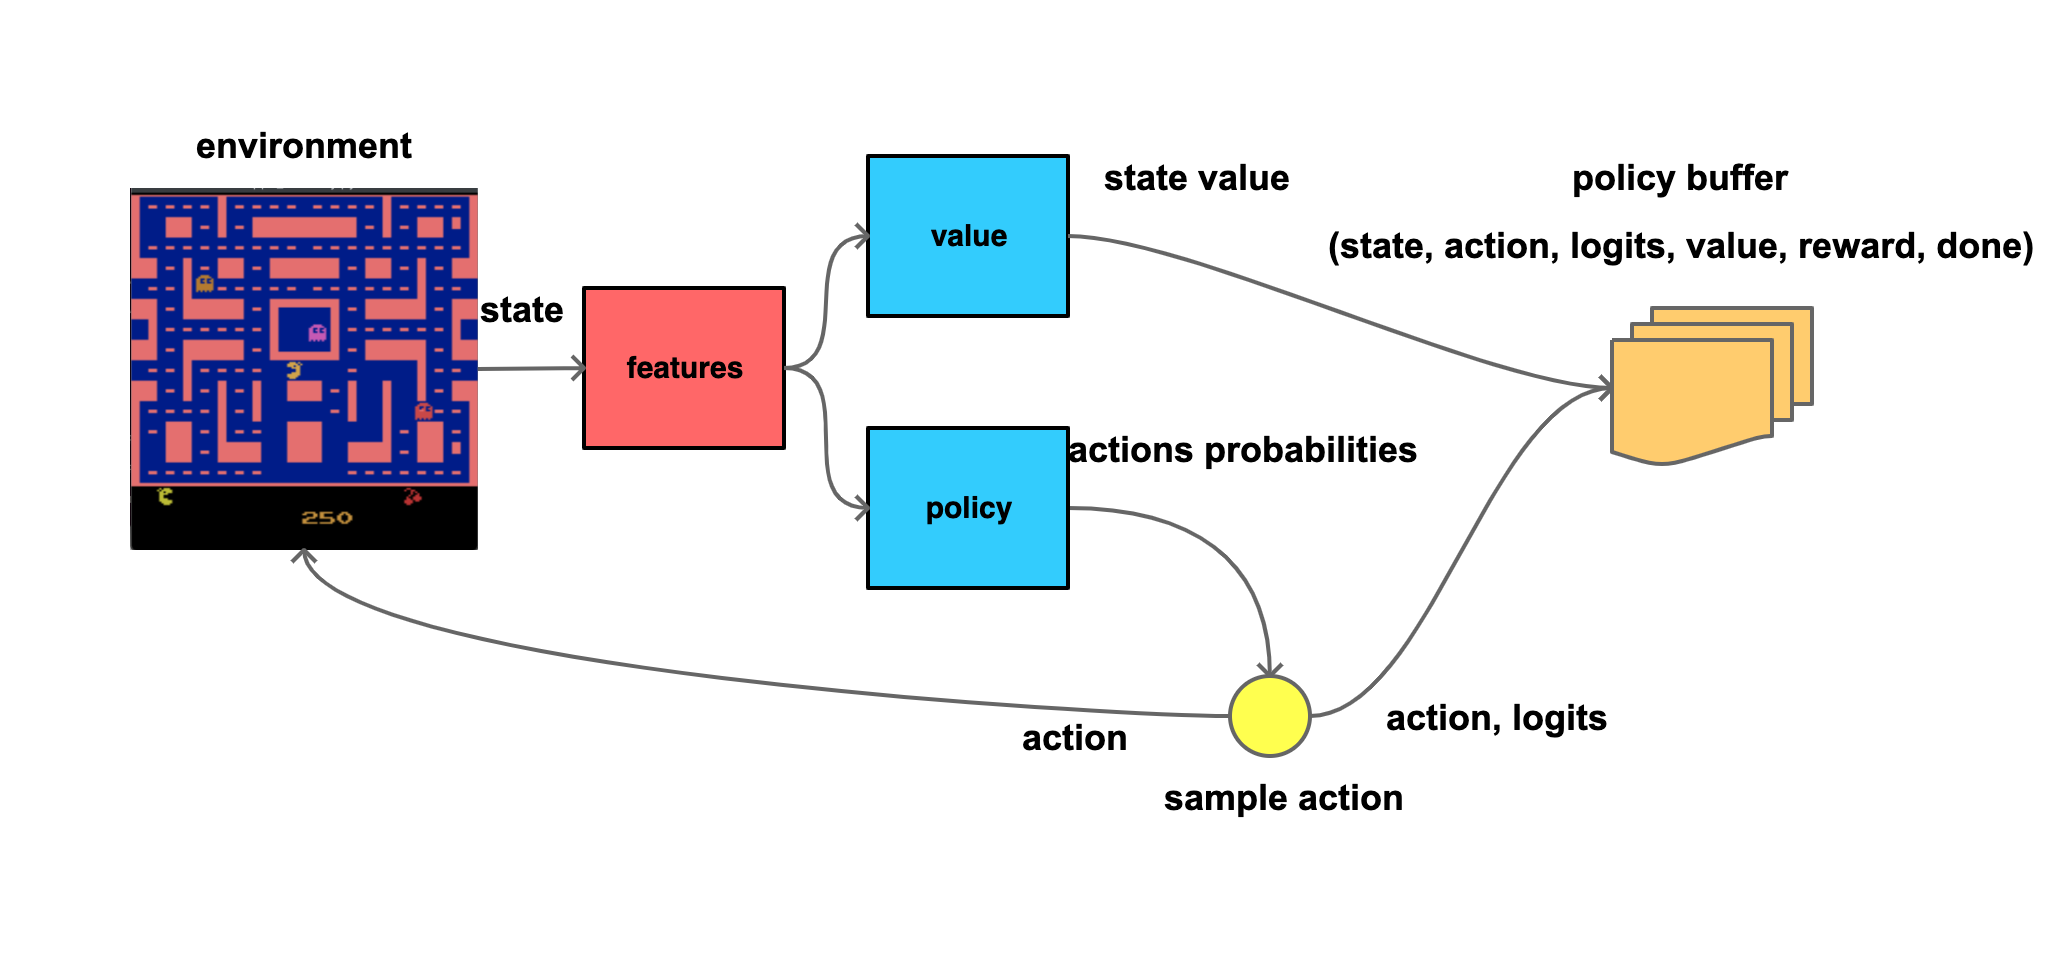
\includegraphics[scale=0.1]{../diagrams/basic/ppo.png}

  
  naive Actor-Critic vs PPO loss: 
  \begin{align*}
    \mathcal{L(\theta)} &= -log \pi(a_n \vert s_n ; \theta) \Big( R(s_n, a_n) - V(s_n) \Big) - \beta\mathcal{H(\pi)} \\
    \mathcal{L(\theta)} &= -log \frac{\pi(a_n \vert s_n ; \theta)}{\pi(a_n \vert s_n ; \theta_{old})} \Big( R(s_n, a_n) - V(s_n) \Big) - \beta\mathcal{H(\pi)} \\
  \end{align*} 

\end{frame}



\begin{frame}{\bf Montezuma's Revenge}

  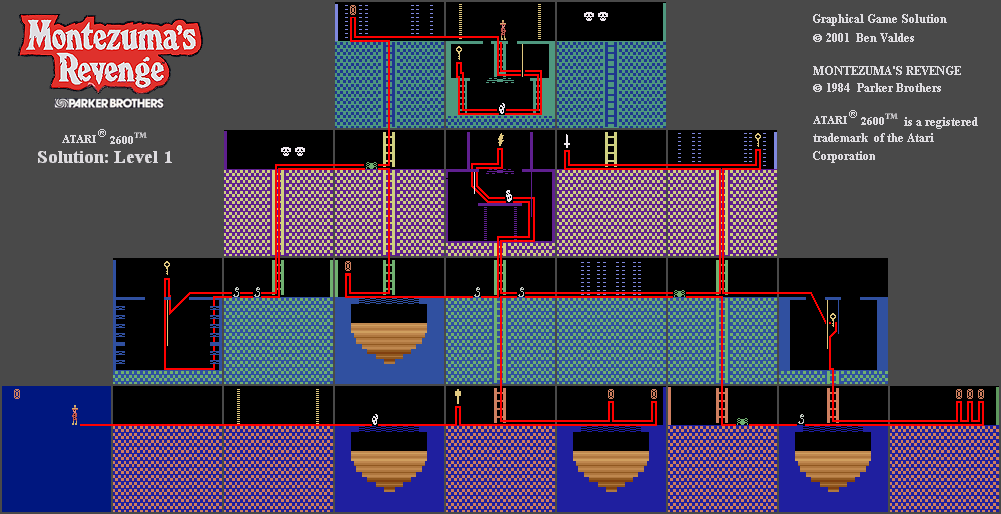
\includegraphics[scale=0.32]{../images/montezuma_map.png}
  
  \end{frame}
  
  \begin{frame}{\bf Montezuma's Revenge}
  
    \begin{columns}
  
      \begin{column}{0.5\textwidth}
        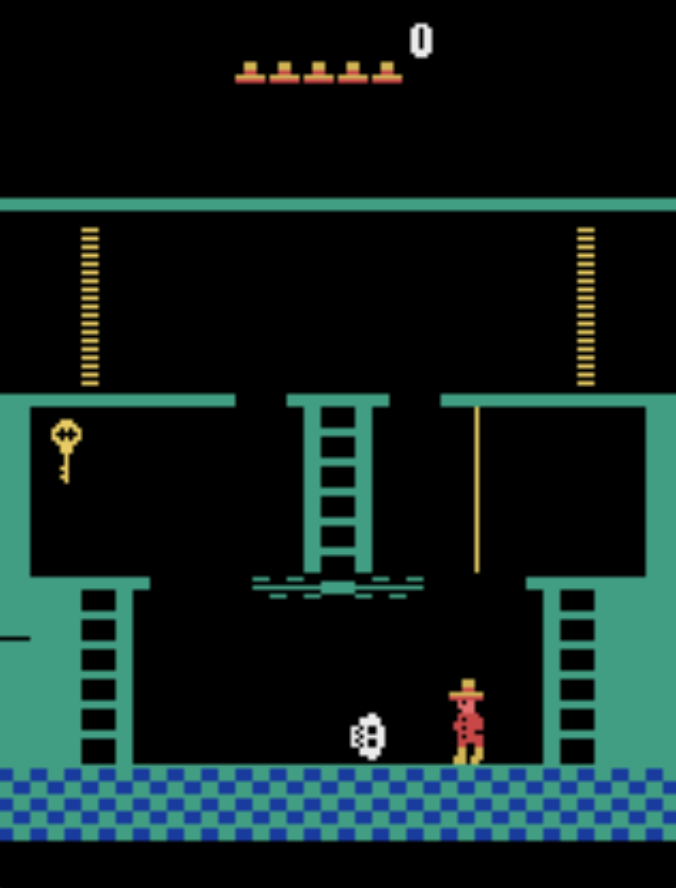
\includegraphics[scale=0.32]{../images/montezuma.png}
      \end{column}
  
      \begin{column}{0.5\textwidth}
        \begin{itemize}
          \item {\bf very sparse rewards} - hundrets of steps
          \item {\bf huge state space}
          \item {\bf hard exploration}
          \item {\bf needs returns back}
        \end{itemize}
      \end{column}
  
  
    \end{columns}
  
  \end{frame}
  
  
  \begin{frame}{\bf state of the art score}
  
  
  \begin{columns}
      \column{\dimexpr\paperwidth-10pt}
  
        source : \url{https://paperswithcode.com/sota/atari-games-on-atari-2600-montezumas-revenge}
  
  
        \begin{table}[]
        \begin{tabular}{|l|l|l|}
        \hline
        \textbf{year} & \textbf{name}                                       & \textbf{score} \\ \hline
        2015          & Deep Reinforcement Learning with Double Q-learning  & 0              \\ \hline
        2017          & Curiosity-driven Exploration by Self-supervised Prediction \footnote[1]{https://arxiv.org/abs/1705.05363} & 0       \\ \hline 
        2021          & MuZero                                              & 2500           \\ \hline
        2018          & Count-Based Exploration with Neural Density Models \footnote[2]{https://arxiv.org/abs/1703.01310}  & 3705           \\ \hline
        \textbf{2019} & \textbf{Exploration by Random Network Distillation} \footnote[3]{https://arxiv.org/abs/1810.12894}& \textbf{8152}  \\ \hline
        2021          & GoExplore$^*$ \footnote[4]{https://arxiv.org/abs/2004.12919}                         & 43 000         \\ \hline
        \end{tabular}
        \end{table}
  
        {\bf * requires environment state saving/loading}
  
  \end{columns}
  
  
  \end{frame}
  
  
  \begin{frame}{\bf state of the art score}
  
  \centering
  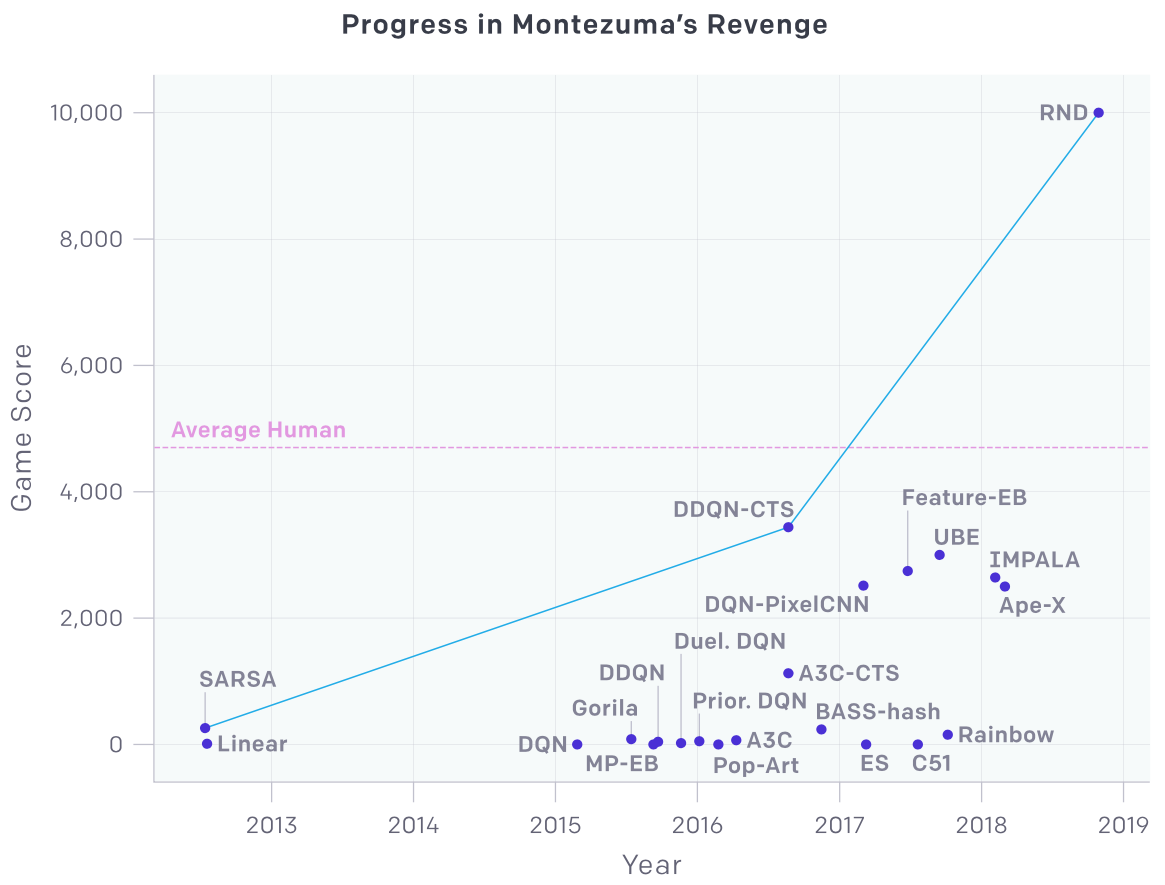
\includegraphics[scale=0.2]{../images/montezuma_progress.png}
  
  
\end{frame}



\begin{frame}
  
  \frametitle{why so hard ?} 

  {Investigating Human Priors for Playing Video Games \footnote{\href{https://arxiv.org/pdf/1802.10217.pdf}{Dubey et al. 2018}} }

  \centering
  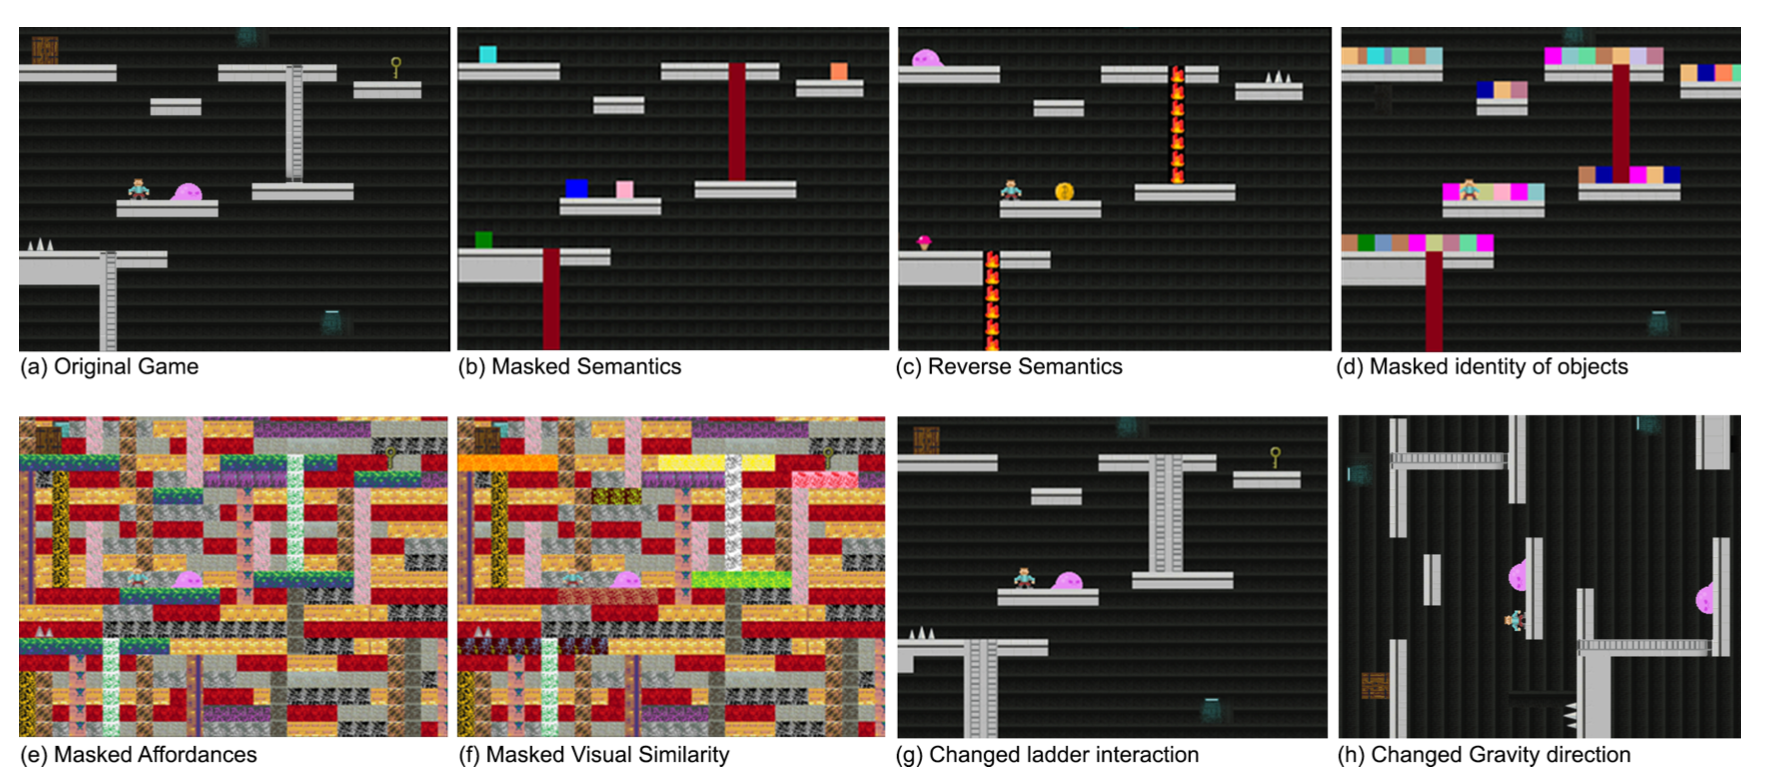
\includegraphics[scale=0.25]{../papers_captions/human_priors_0.png}
  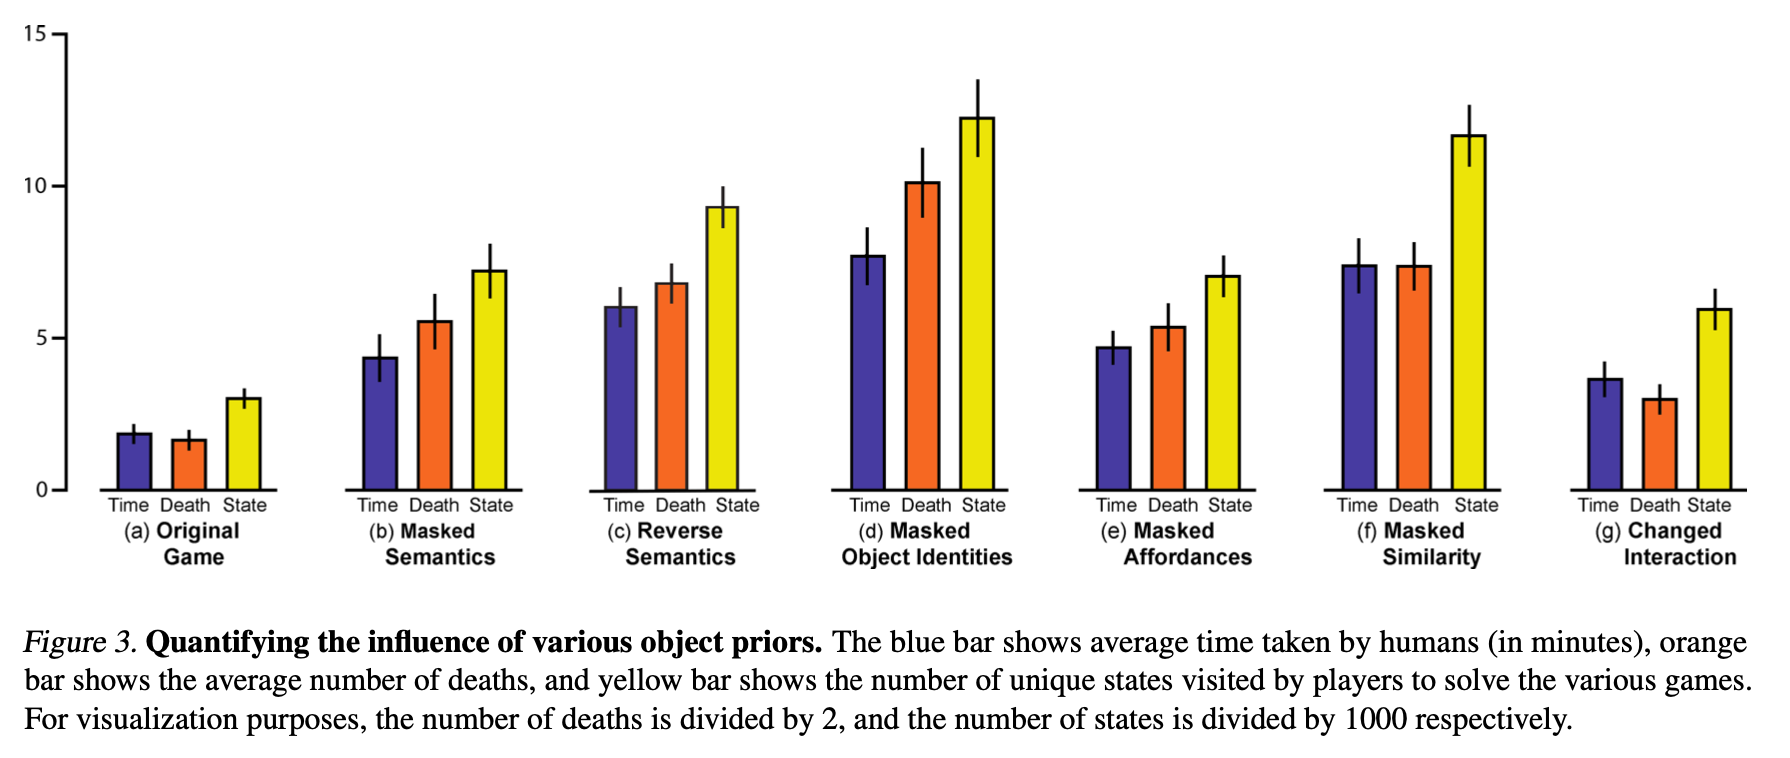
\includegraphics[scale=0.25]{../papers_captions/human_priors_1.png}
  
\end{frame}


\begin{frame}
  \frametitle{problems} 

  \begin{itemize}
    \item hard exploration tasks (sparse rewards)
    \item generalisation
    \item sample efficiency 
  \end{itemize}

\end{frame}


  \begin{frame}{\bf pixel change motivation}

  \centering
  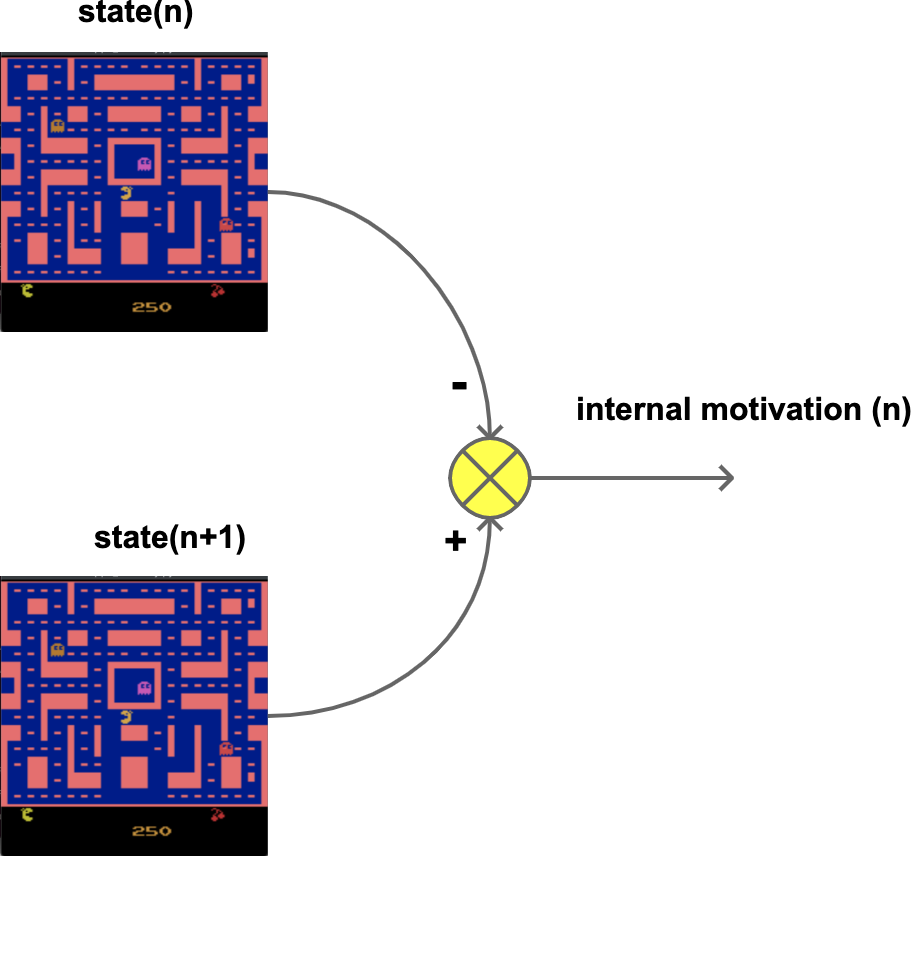
\includegraphics[scale=0.15]{../diagrams/internal_motivation/pixelchange.png}
  
  \end{frame}
  
  
  \begin{frame}{\bf next state prediction}
  
  \centering
  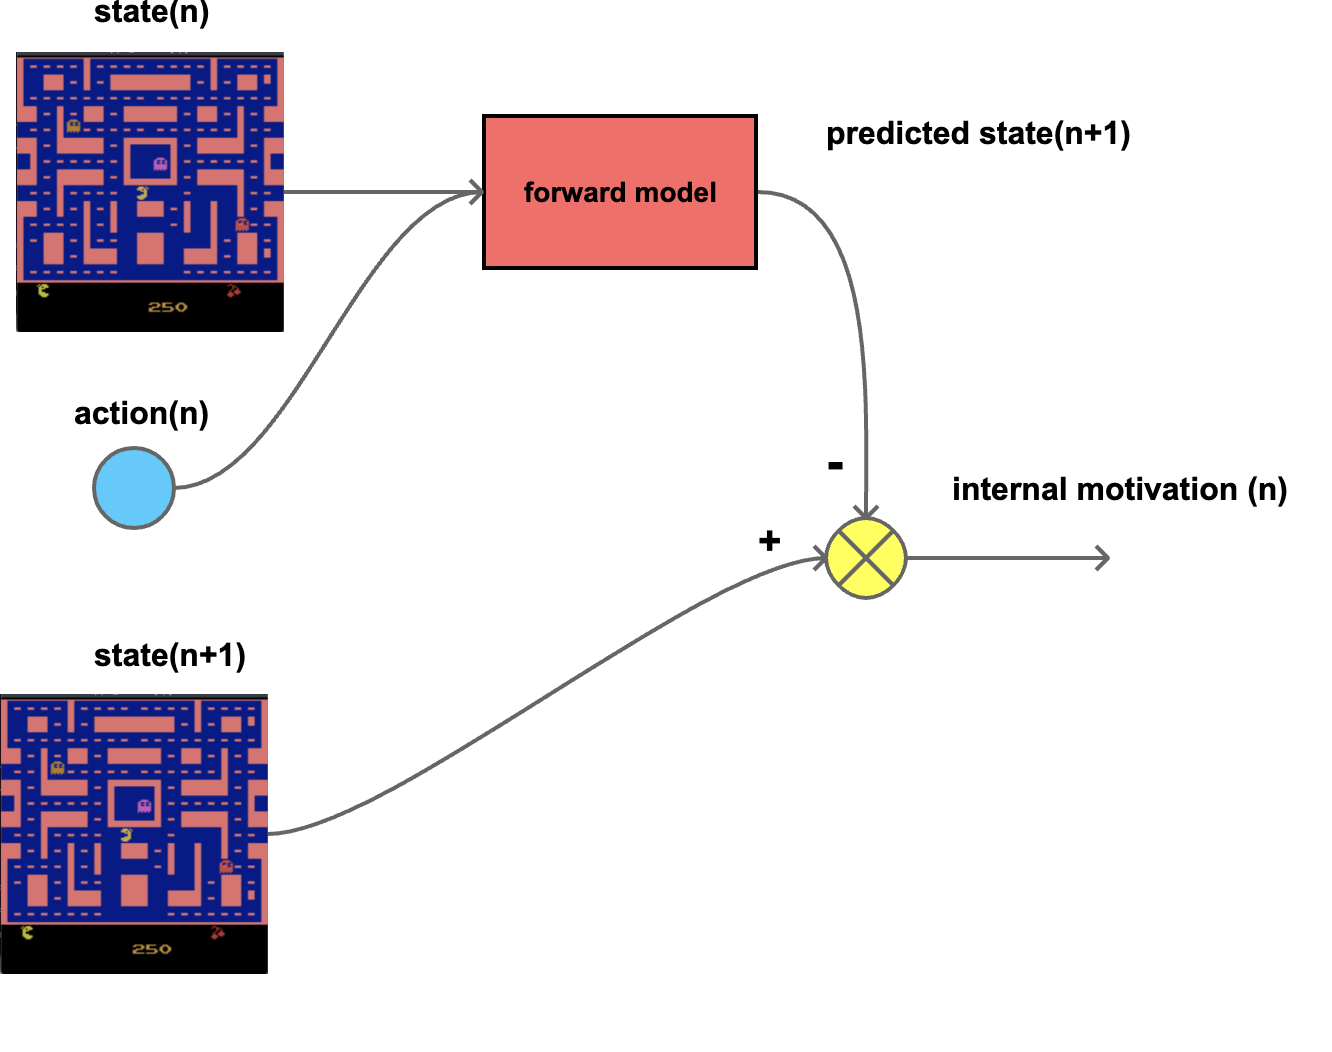
\includegraphics[scale=0.15]{../diagrams/internal_motivation/naive.png}
  
  \end{frame}
  
  
  \begin{frame}
  
    \frametitle{Curiosity-driven Exploration by Self-supervised Prediction
                \footnote{\href{https://arxiv.org/pdf/1705.05363.pdf}{Pathak et al. 2017}} }
  
      \begin{itemize}
        \item {\bf predict next state}, forward model
        \item {\bf motivation == prediction error}
        \item not working ...
      \end{itemize}
  
      \begin{columns}
  
        \begin{column}{0.5\textwidth}
          \centering
          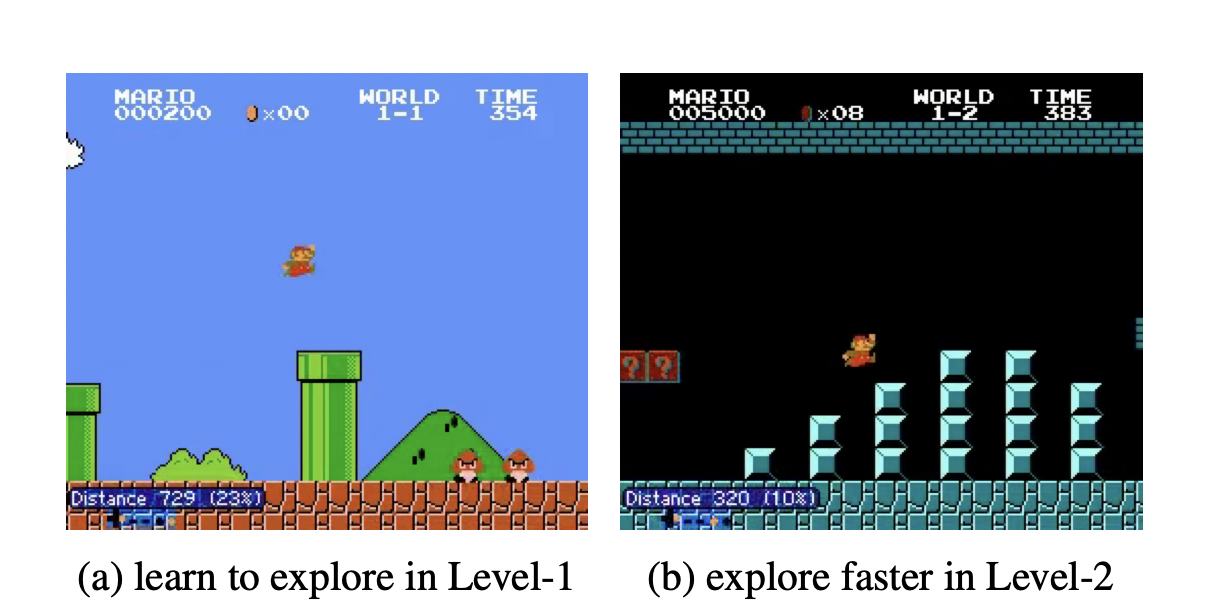
\includegraphics[scale=0.25]{../papers_captions/icm.png}
        \end{column}
  
        \begin{column}{0.5\textwidth}
          \centering
          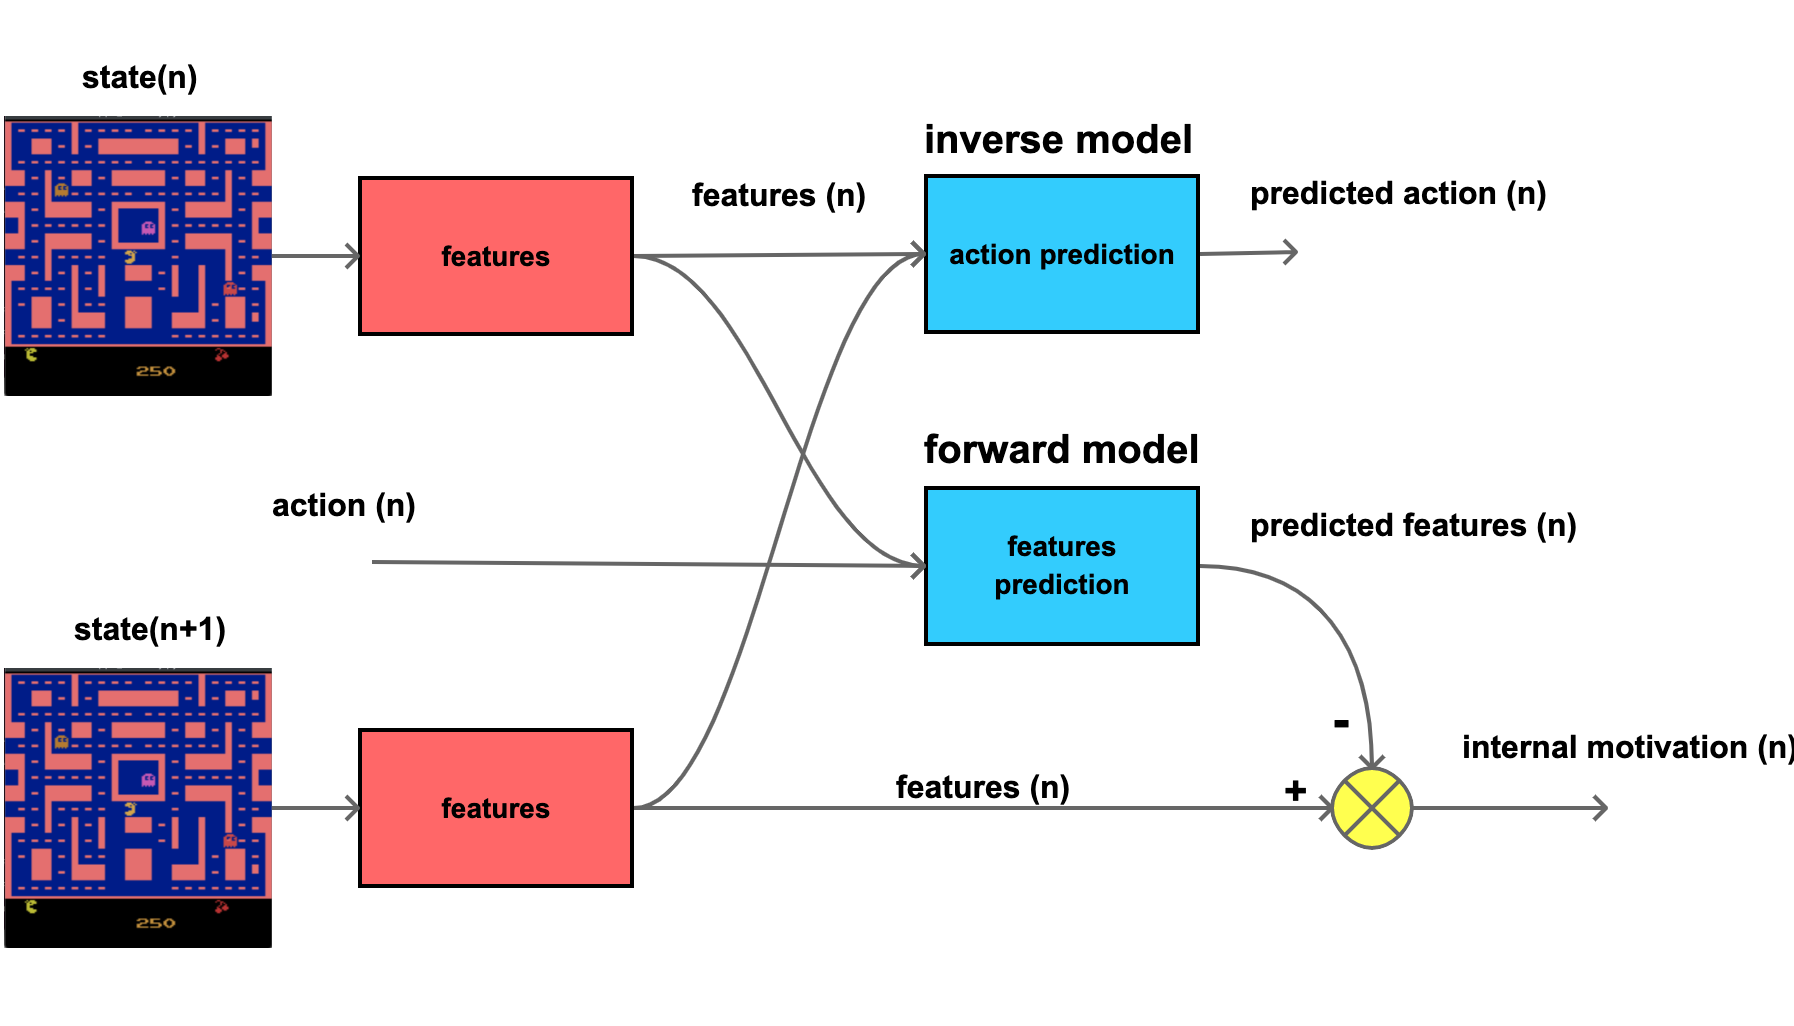
\includegraphics[scale=0.1]{../diagrams/internal_motivation/icm.png}
        \end{column}
      
      \end{columns}
      
  \end{frame}
  
 


  \begin{frame}
  
    \frametitle{Exploration by Random Network Distillation \footnote{\href{https://arxiv.org/pdf/1810.12894.pdf}{Burda et al. 2018}}}
  
    \begin{columns}
  
      
      \begin{column}{0.5\textwidth}
        \centering
        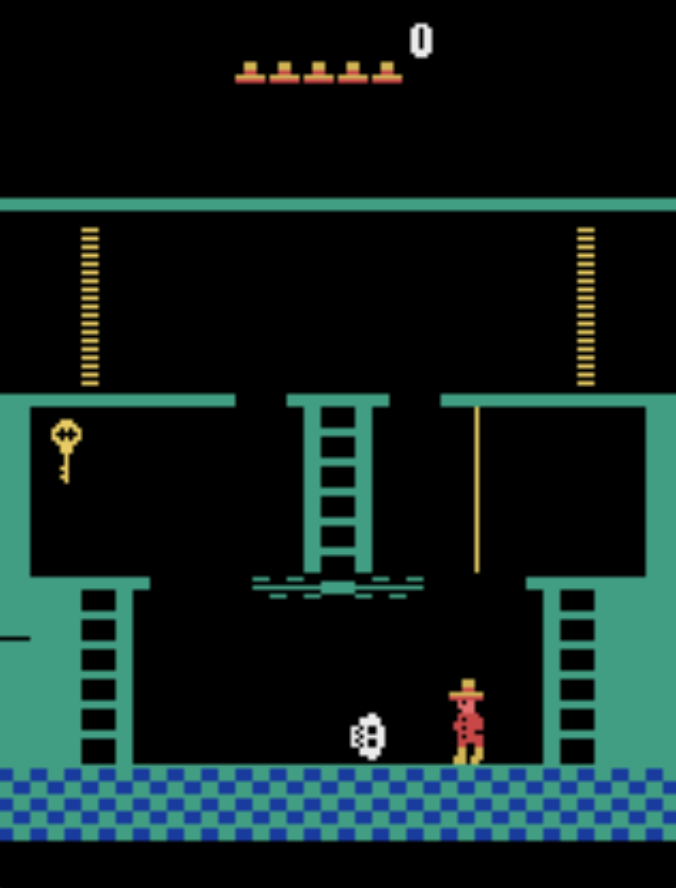
\includegraphics[scale=0.3]{../images/montezuma.png}
      \end{column}

      \begin{column}{0.5\textwidth}
        \centering
        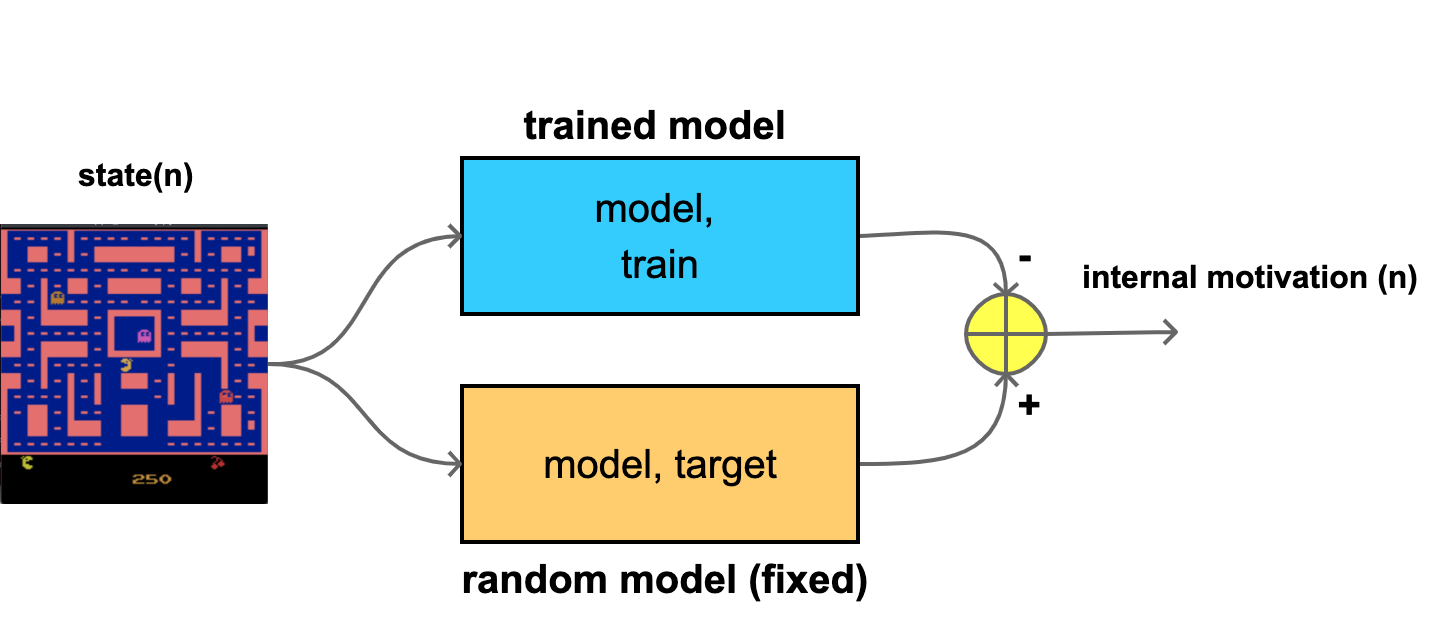
\includegraphics[scale=0.12]{../diagrams/internal_motivation/rnd.png}
      \end{column}
  
    
    \end{columns}
  
  
  \end{frame}
  
  
  
  \begin{frame}{\bf random network distillation}
  
    \begin{columns}
  
      \begin{column}{0.5\textwidth}
        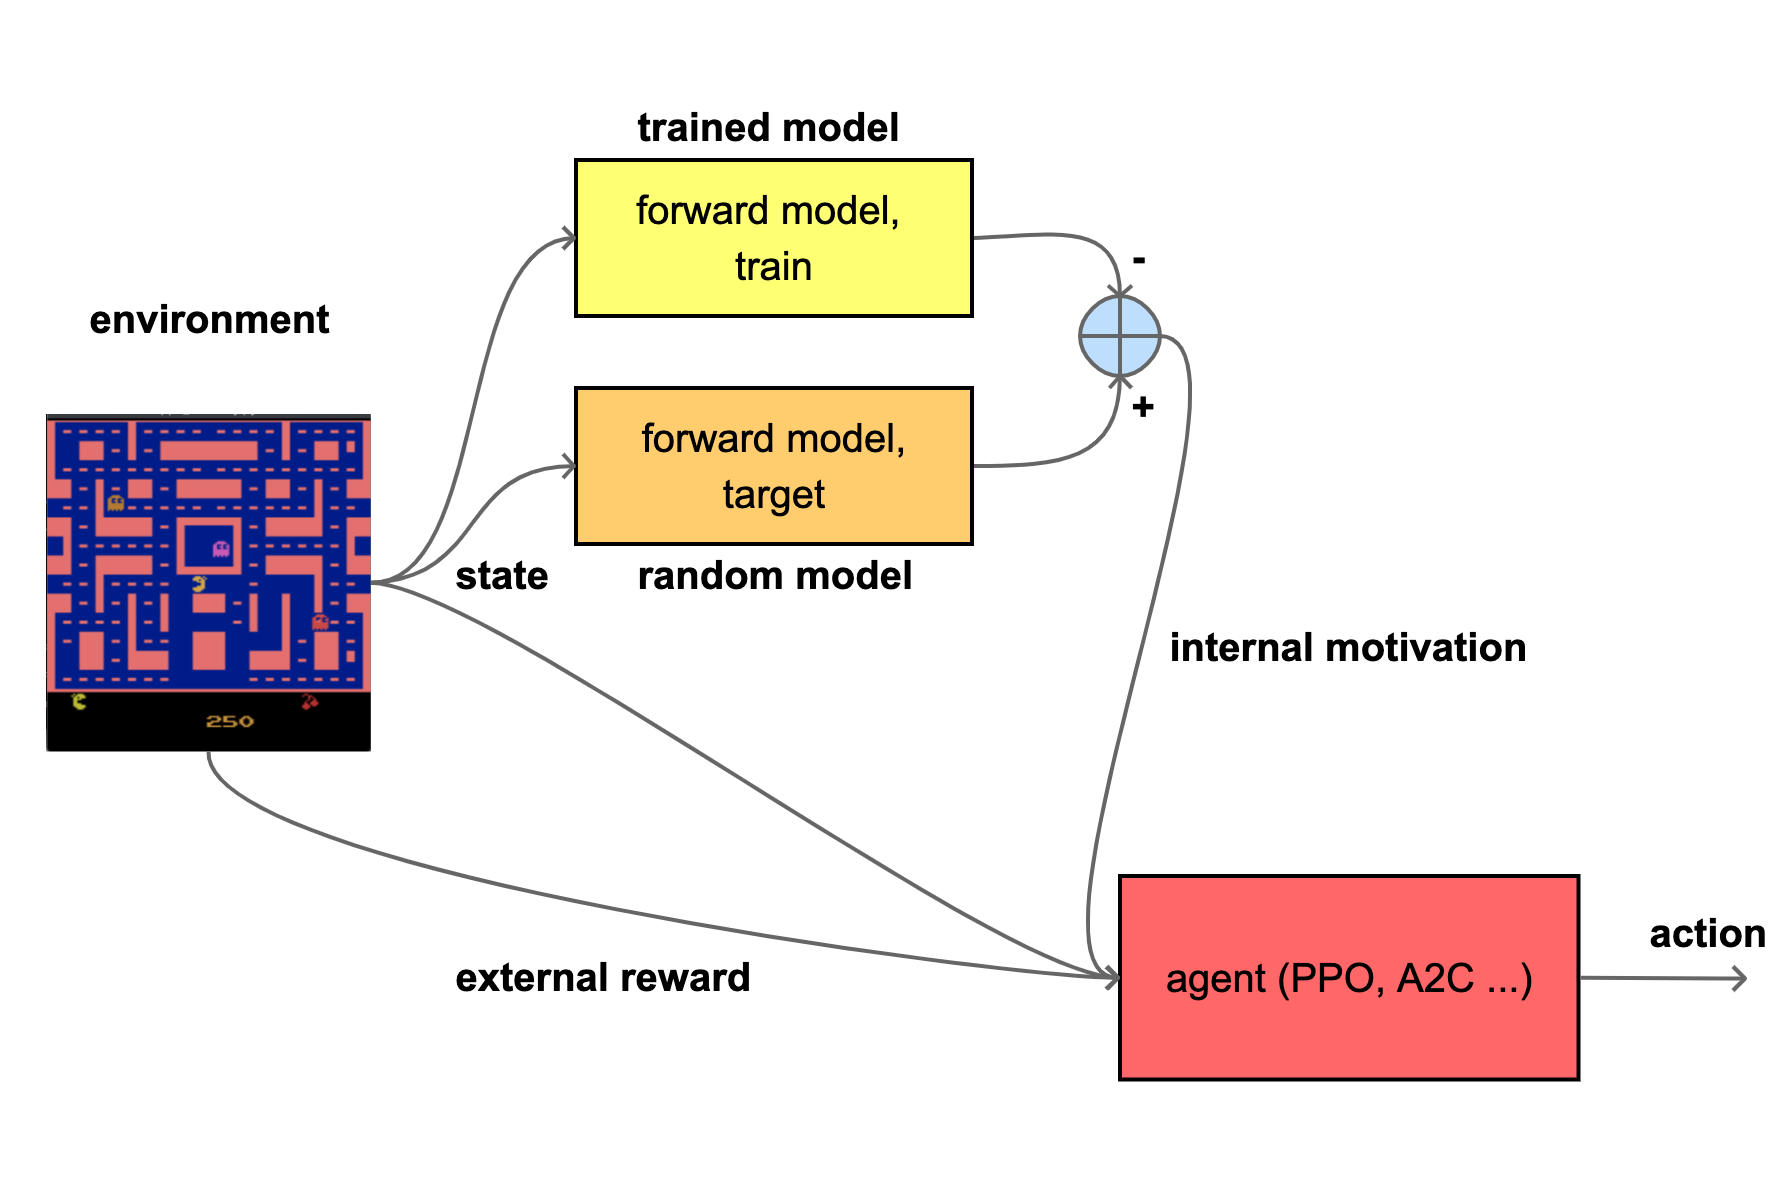
\includegraphics[scale=0.1]{../diagrams/rnd/rnd.png}
      \end{column}
  
      \begin{column}{0.5\textwidth}
        \begin{itemize}
          \item neural network works as {\bf novelty detector}
          \item model learns to imitate random (target) model
          \item {\bf less visited states produce bigger motivation signal}
          \item orthogonal weights initialisation ($g=2^{0.5}$) for strong signal
          \item lot of fully connected layers {\bf to avoid generalisation}
          \item {\bf coupled orthogonal models}
        \end{itemize}
      \end{column}
  
  
    \end{columns}
  
  \end{frame}
  
  
  \begin{frame}{\bf random network distillation architecture}
  
  \centering
  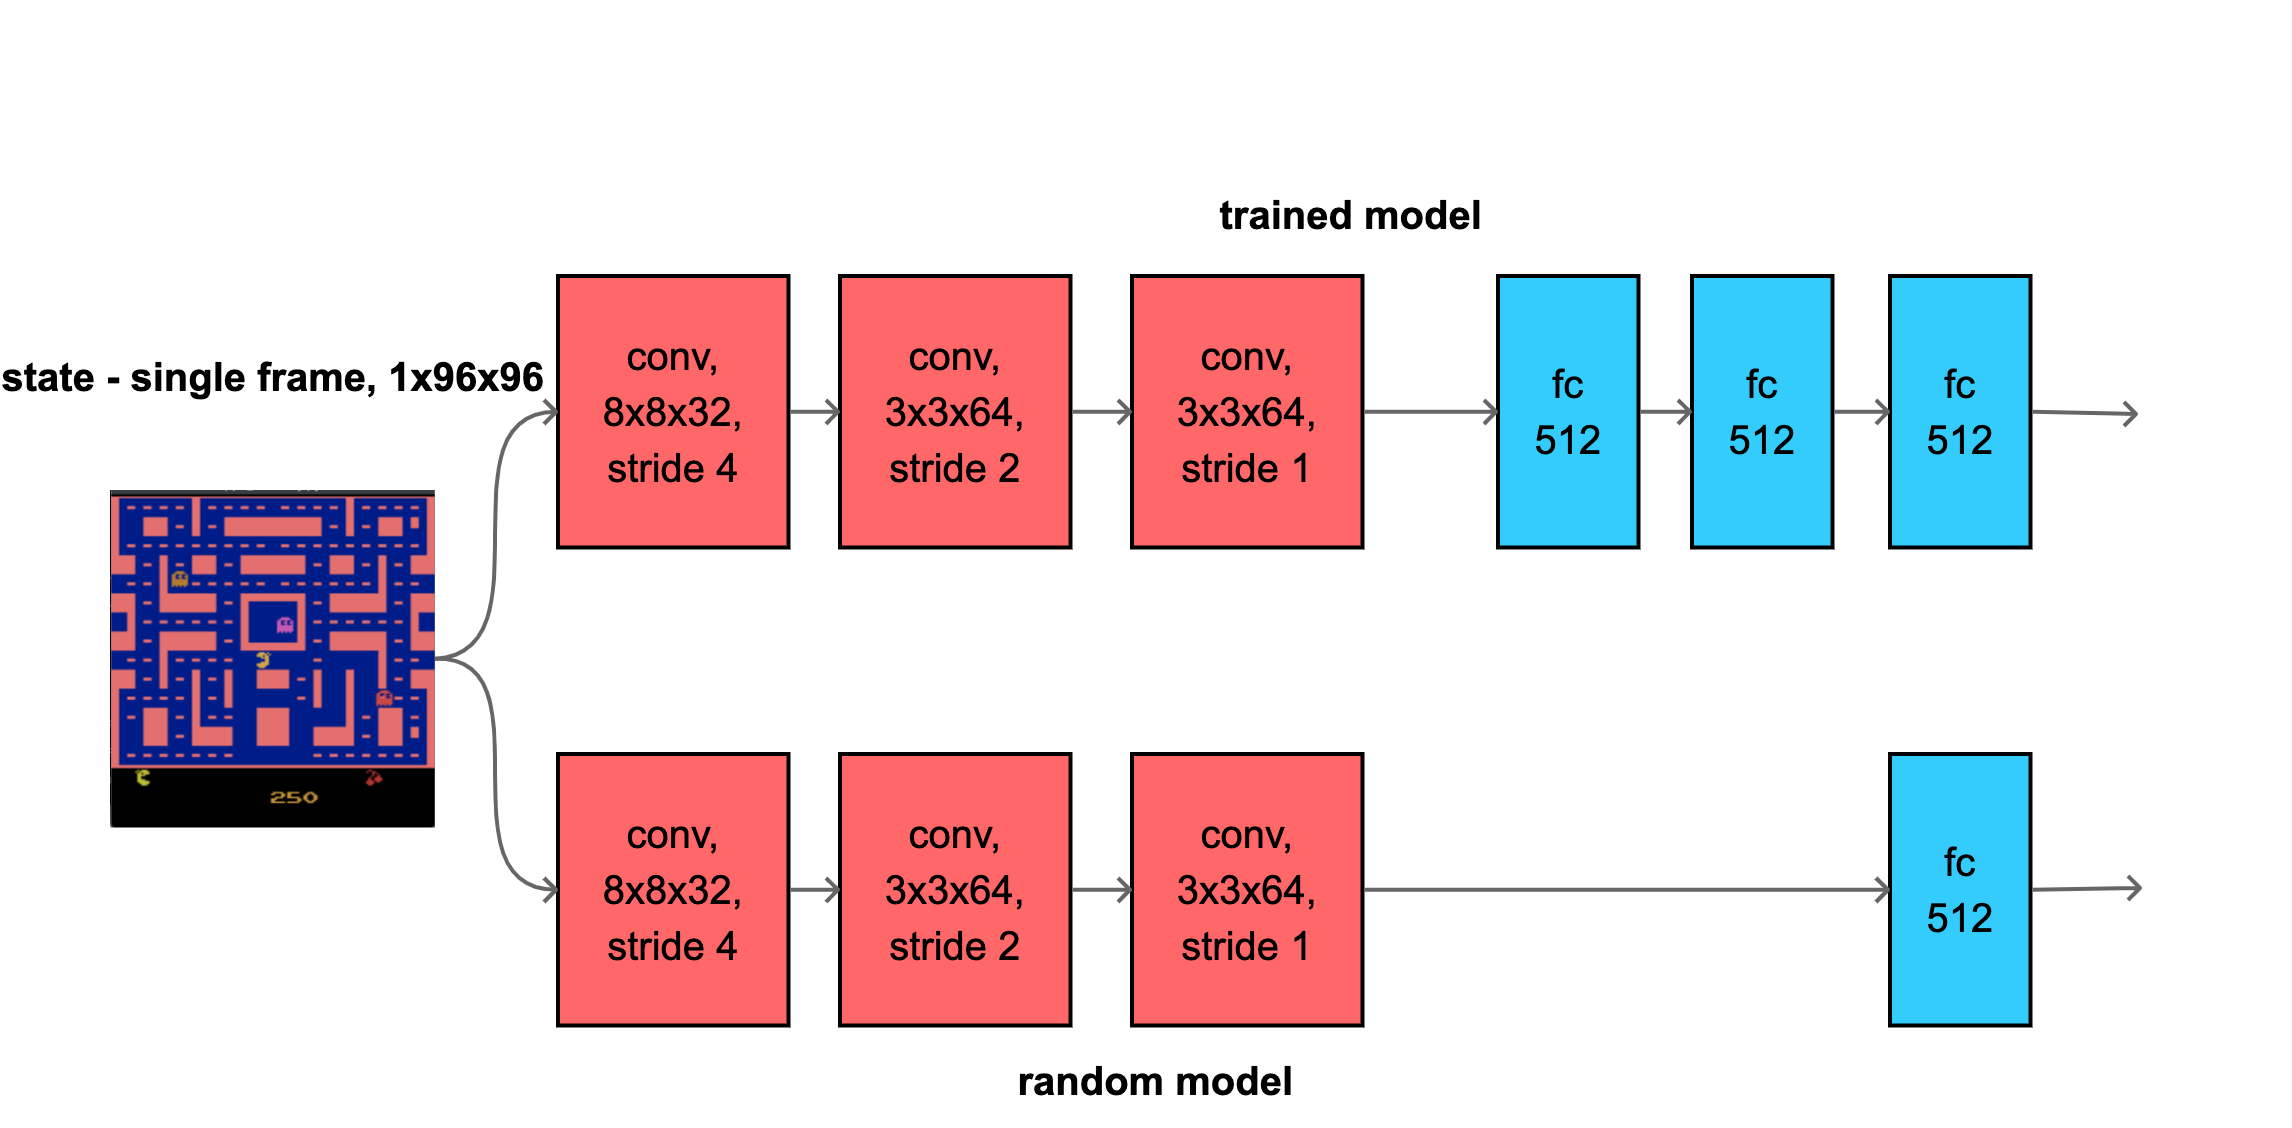
\includegraphics[scale=0.12]{../diagrams/rnd/modelrnd.png}
  
  \end{frame}


  \begin{frame}{\bf coupled RND architecture}
  
    \begin{columns}
    
        \begin{column}{0.5\textwidth}
          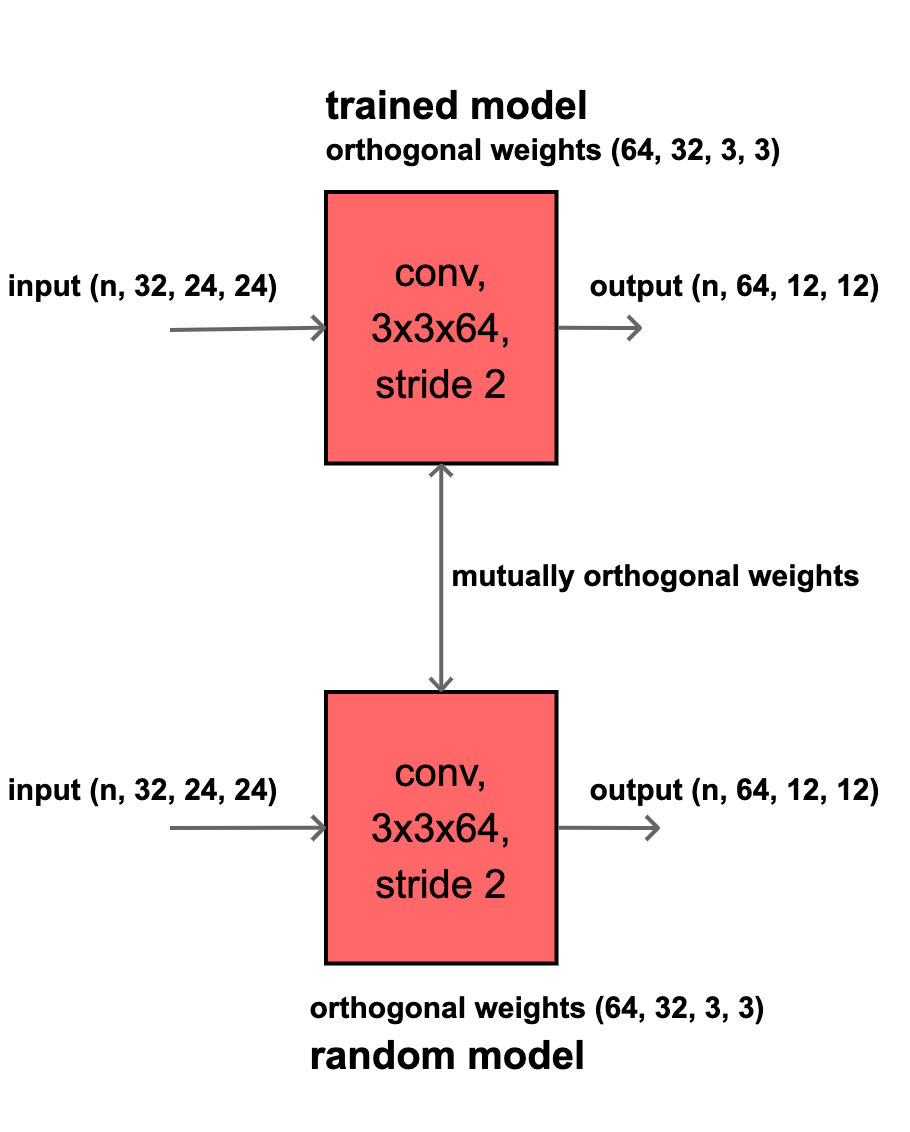
\includegraphics[scale=0.18]{../diagrams/rnd/coupledrnd.png}
        \end{column}
    
        \begin{column}{0.5\textwidth}
          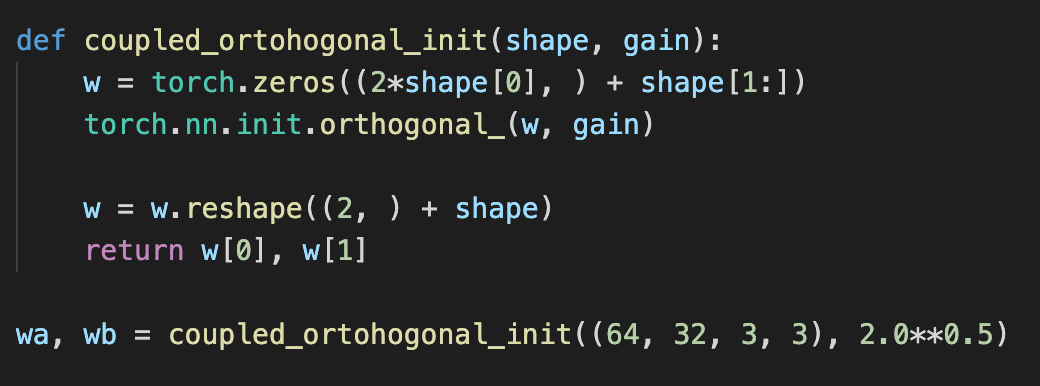
\includegraphics[scale=0.32]{../images/coupled_orthogonal.png}
        \end{column}
    
    \end{columns}
    
  \end{frame}



  \begin{frame}{\bf ppo model architecture}

  \centering
  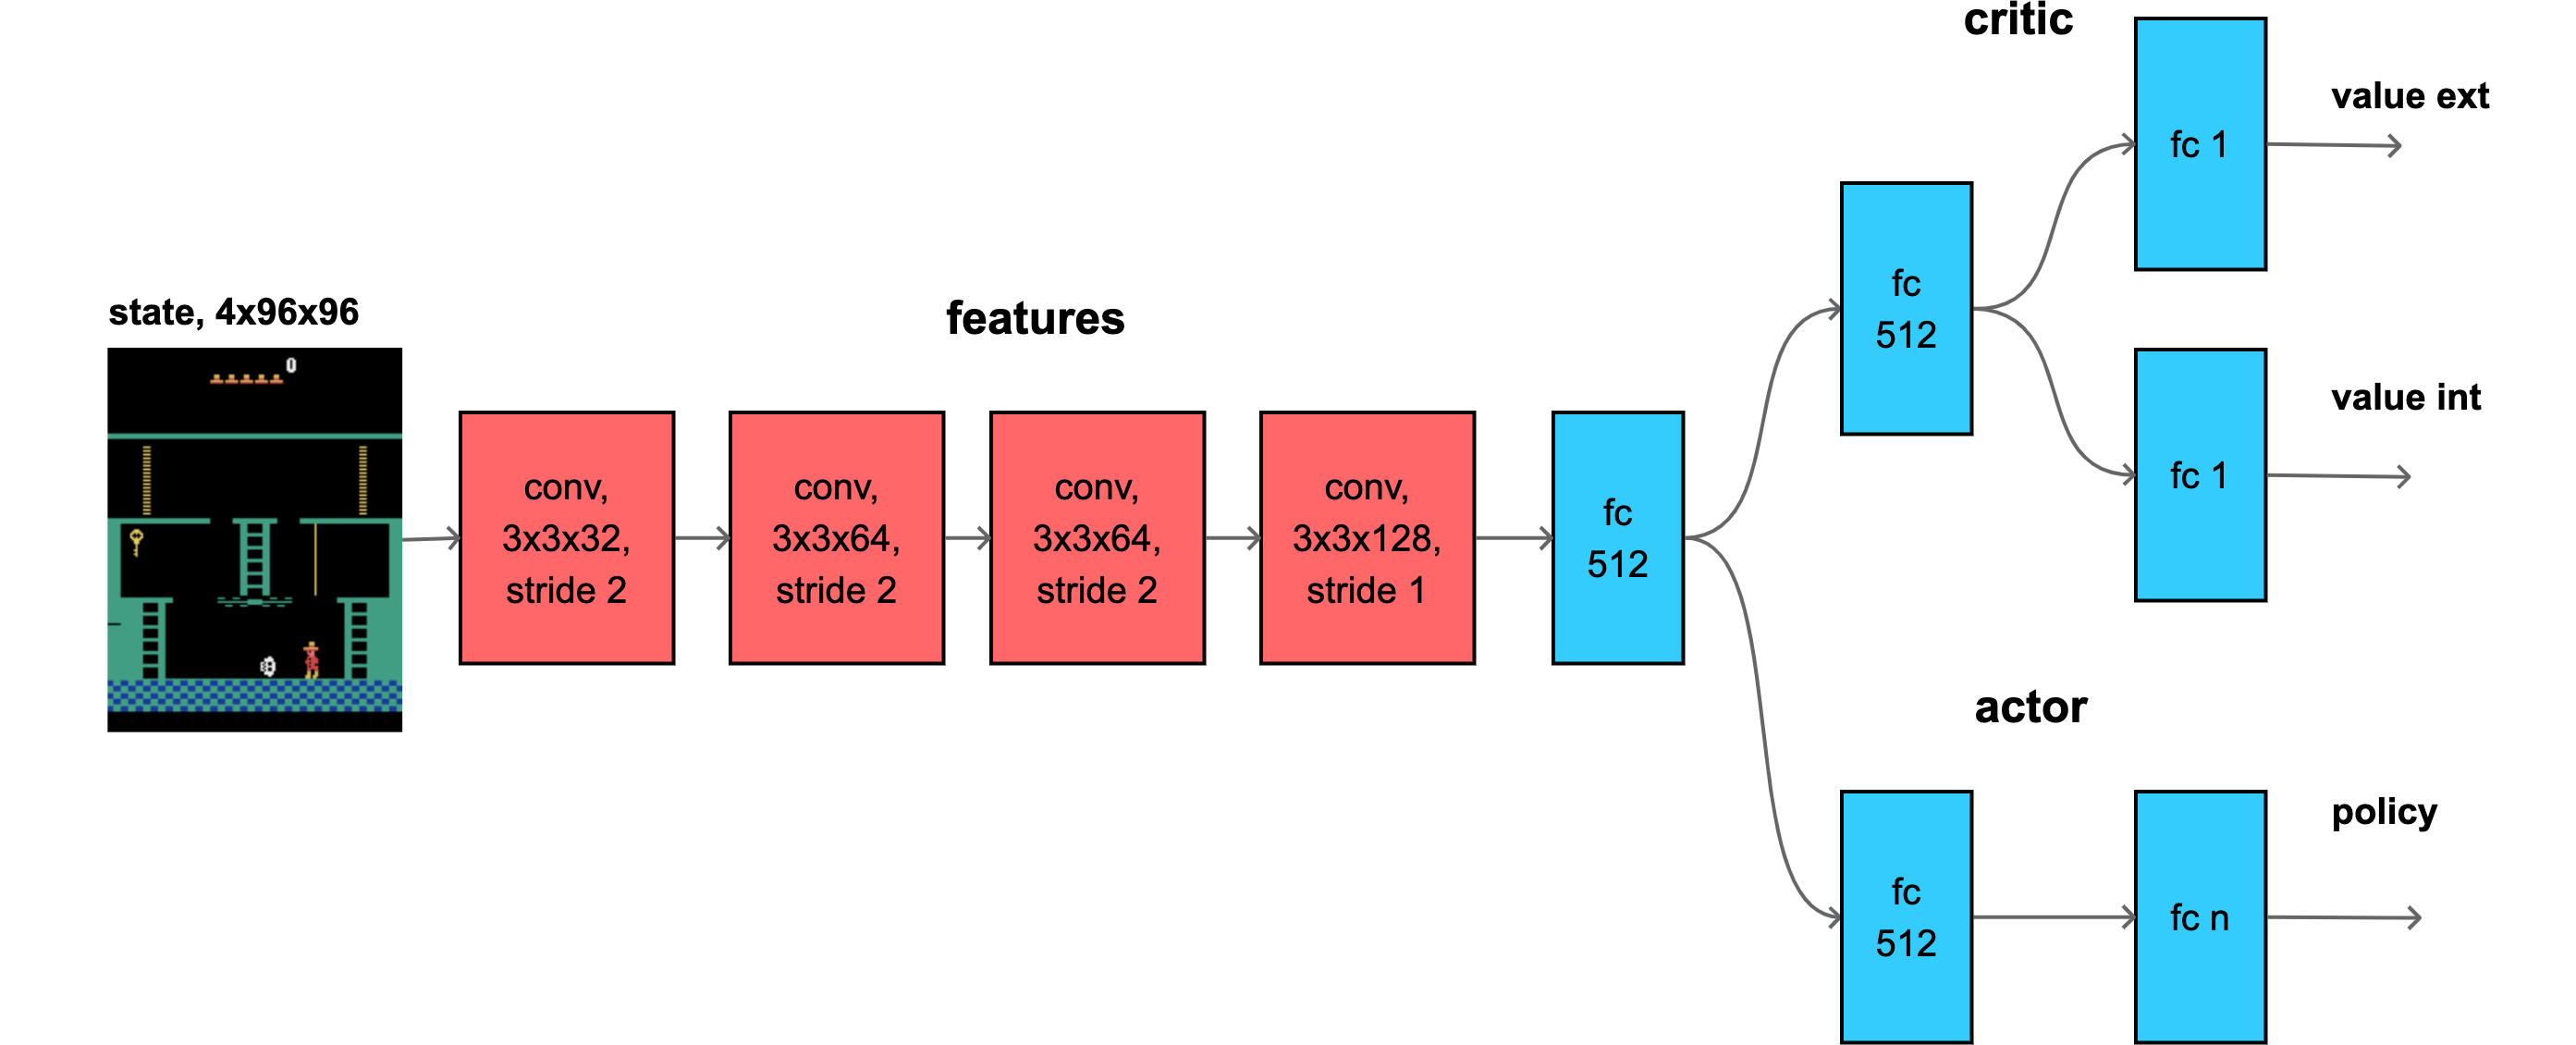
\includegraphics[scale=0.12]{../diagrams/rnd/modelppoc.png}
    
  \end{frame}
  
  
  
  

















\begin{frame}
  
  \frametitle{hide and seek \footnote{\href{https://arxiv.org/pdf/1909.07528.pdf}{Baker et al. 2020}}}
  \href{https://openai.com/blog/emergent-tool-use/}{OpenAI - Emergent Tool Use from Multi-Agent Interaction}

  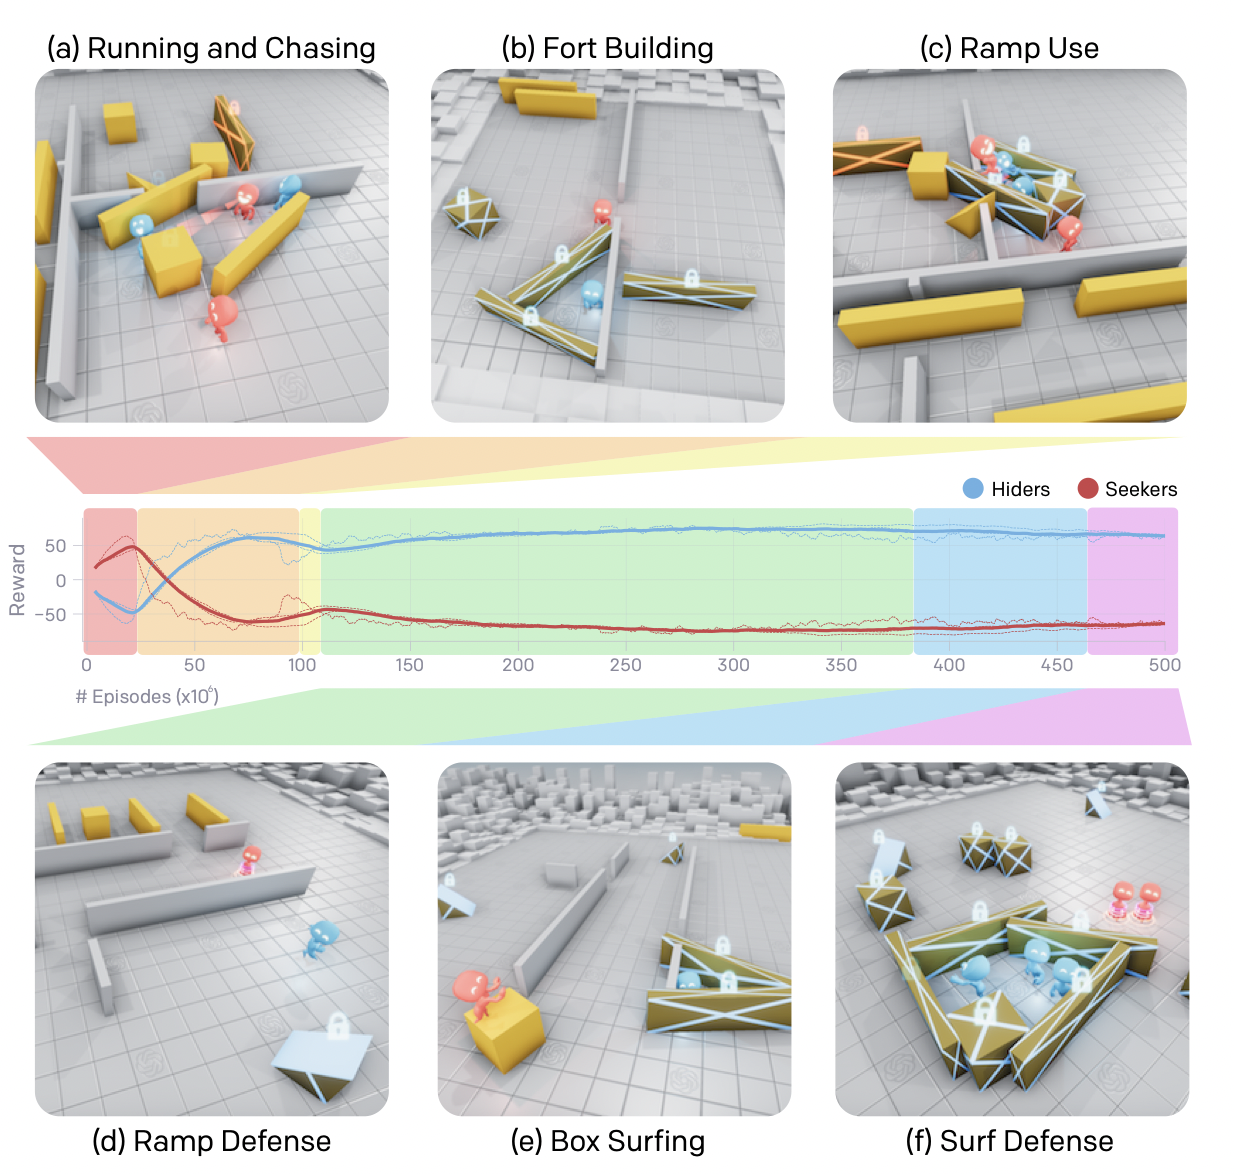
\includegraphics[scale=0.3]{../images/hide_and_seek.png}

\end{frame}



\begin{frame}
  
  \frametitle{generalisation \footnote{\href{https://arxiv.org/pdf/2111.09794.pdf}{Kirk et al. 2021}}}
 
  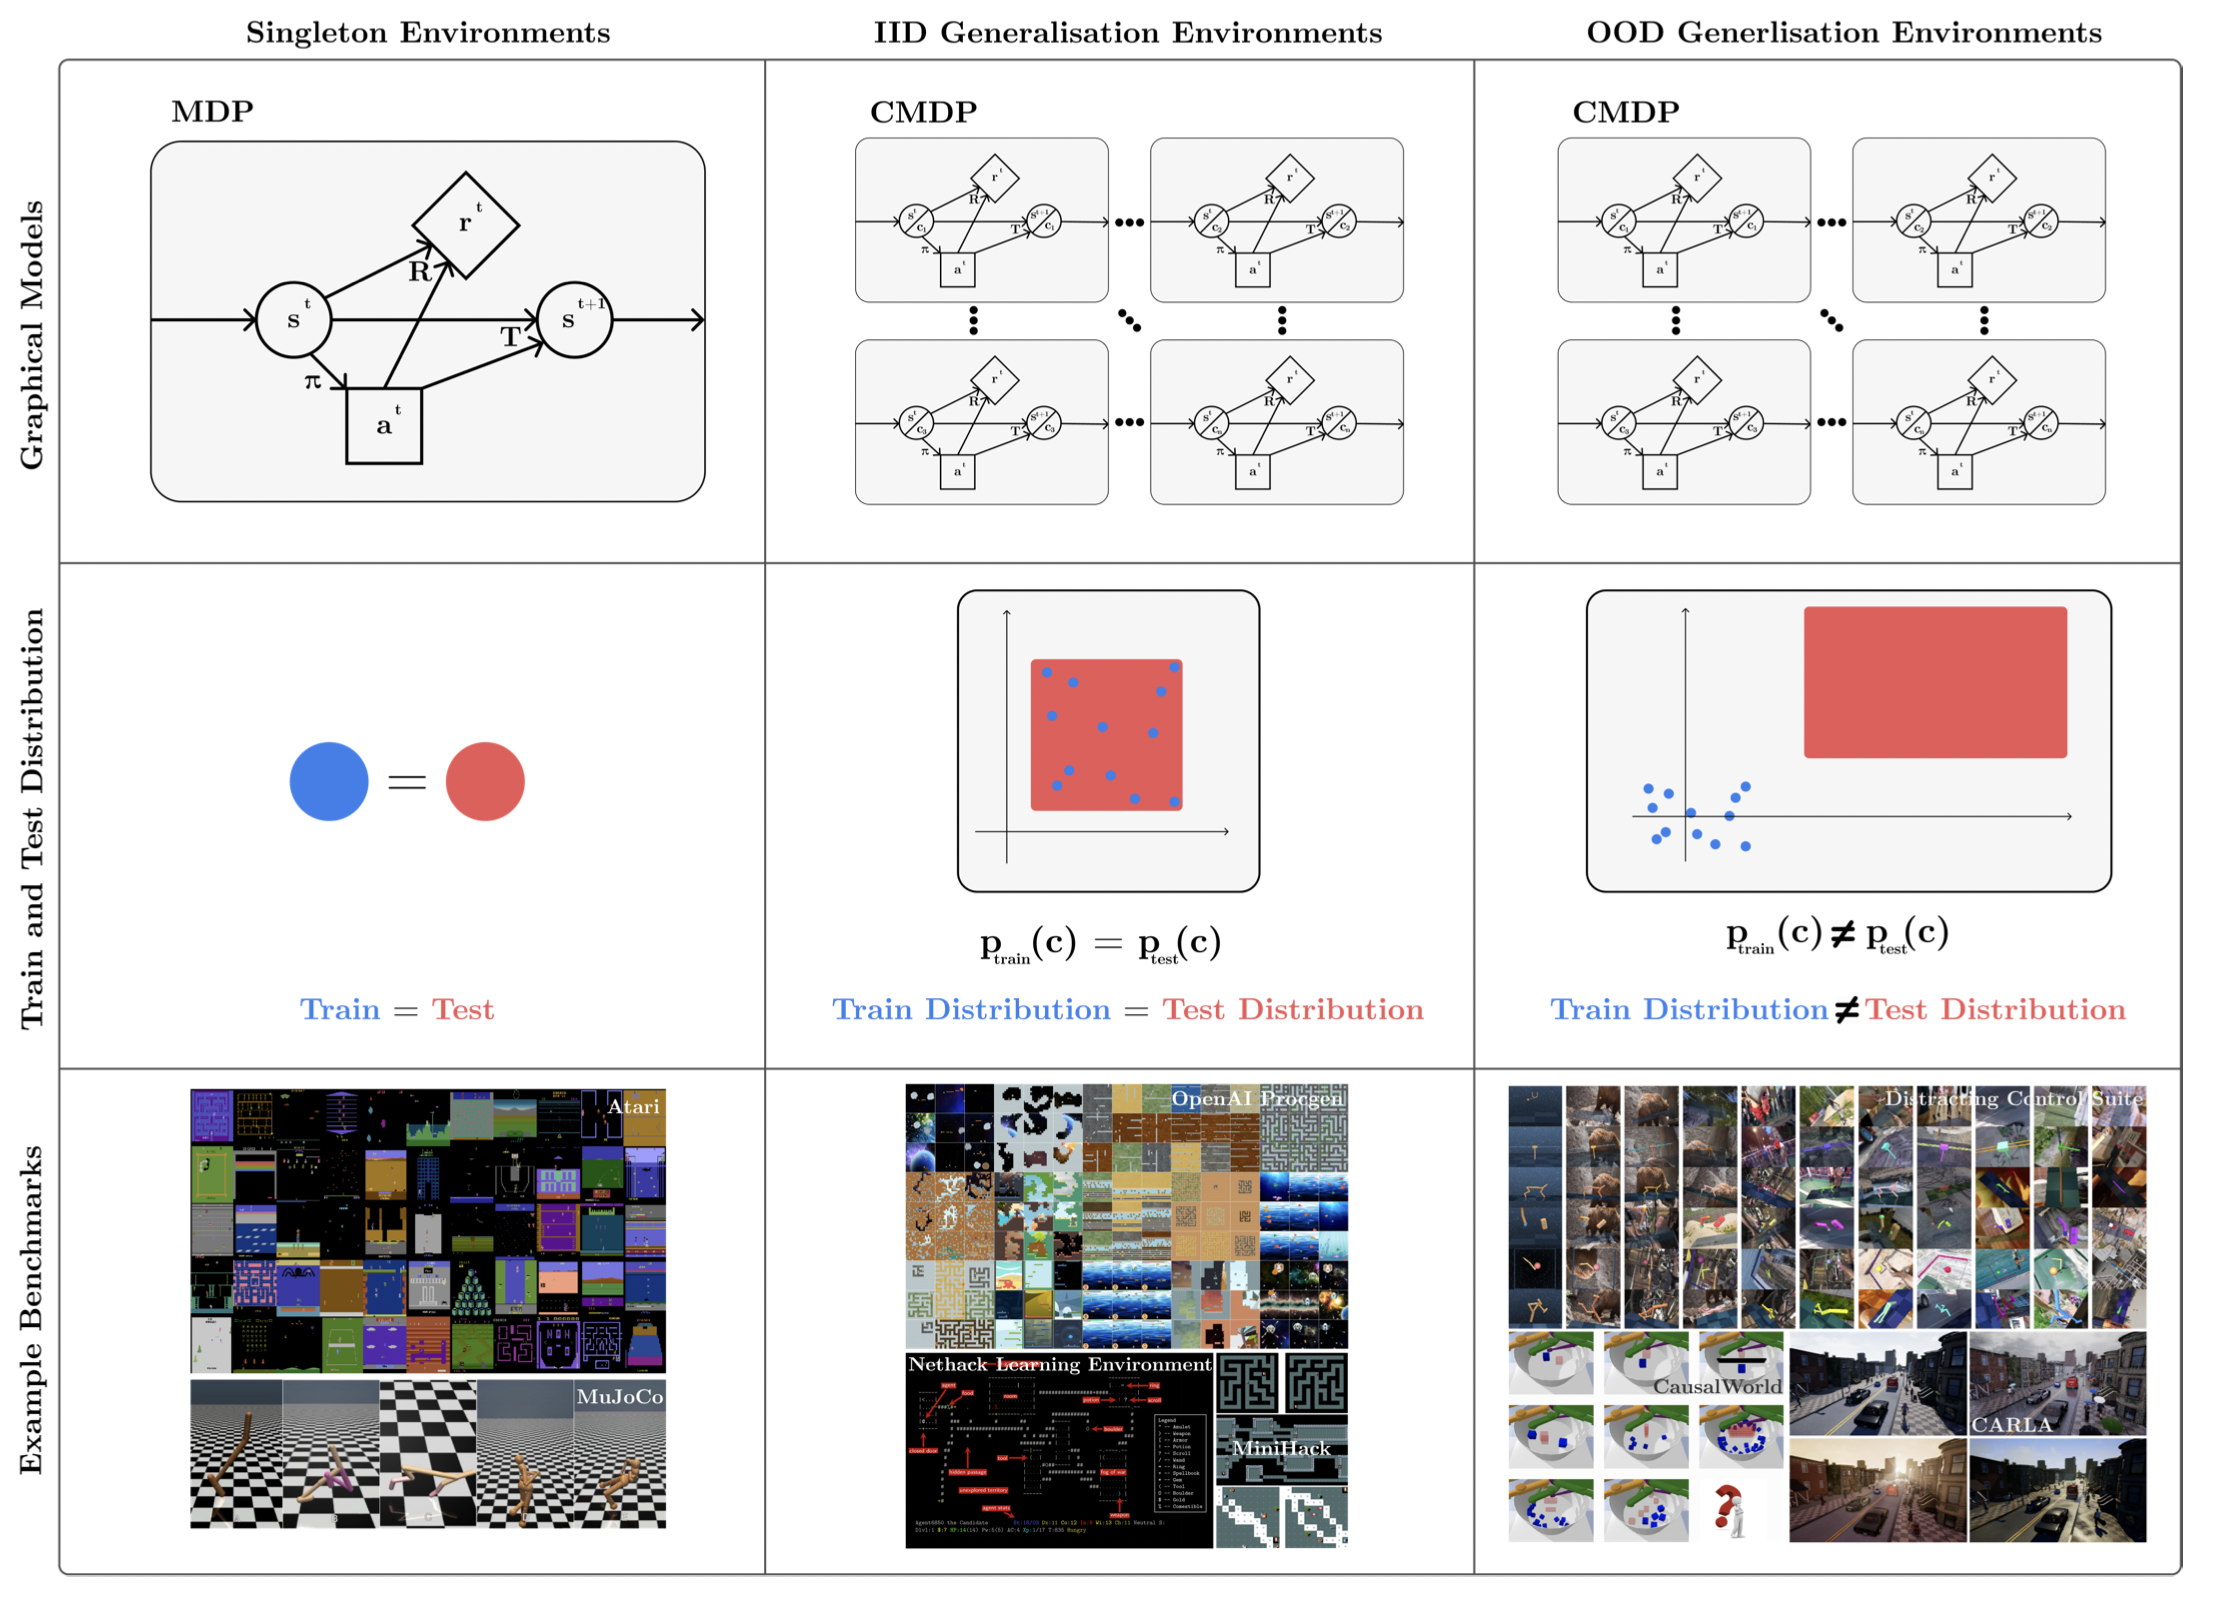
\includegraphics[scale=0.25]{../images/generalisation.png}

\end{frame}


\begin{frame}
  
  \frametitle{RMA: Rapid Motor Adaptation for Legged Robots \footnote{\href{https://arxiv.org/pdf/2107.04034.pdf}{Kumar et al. 2021}}}
 
  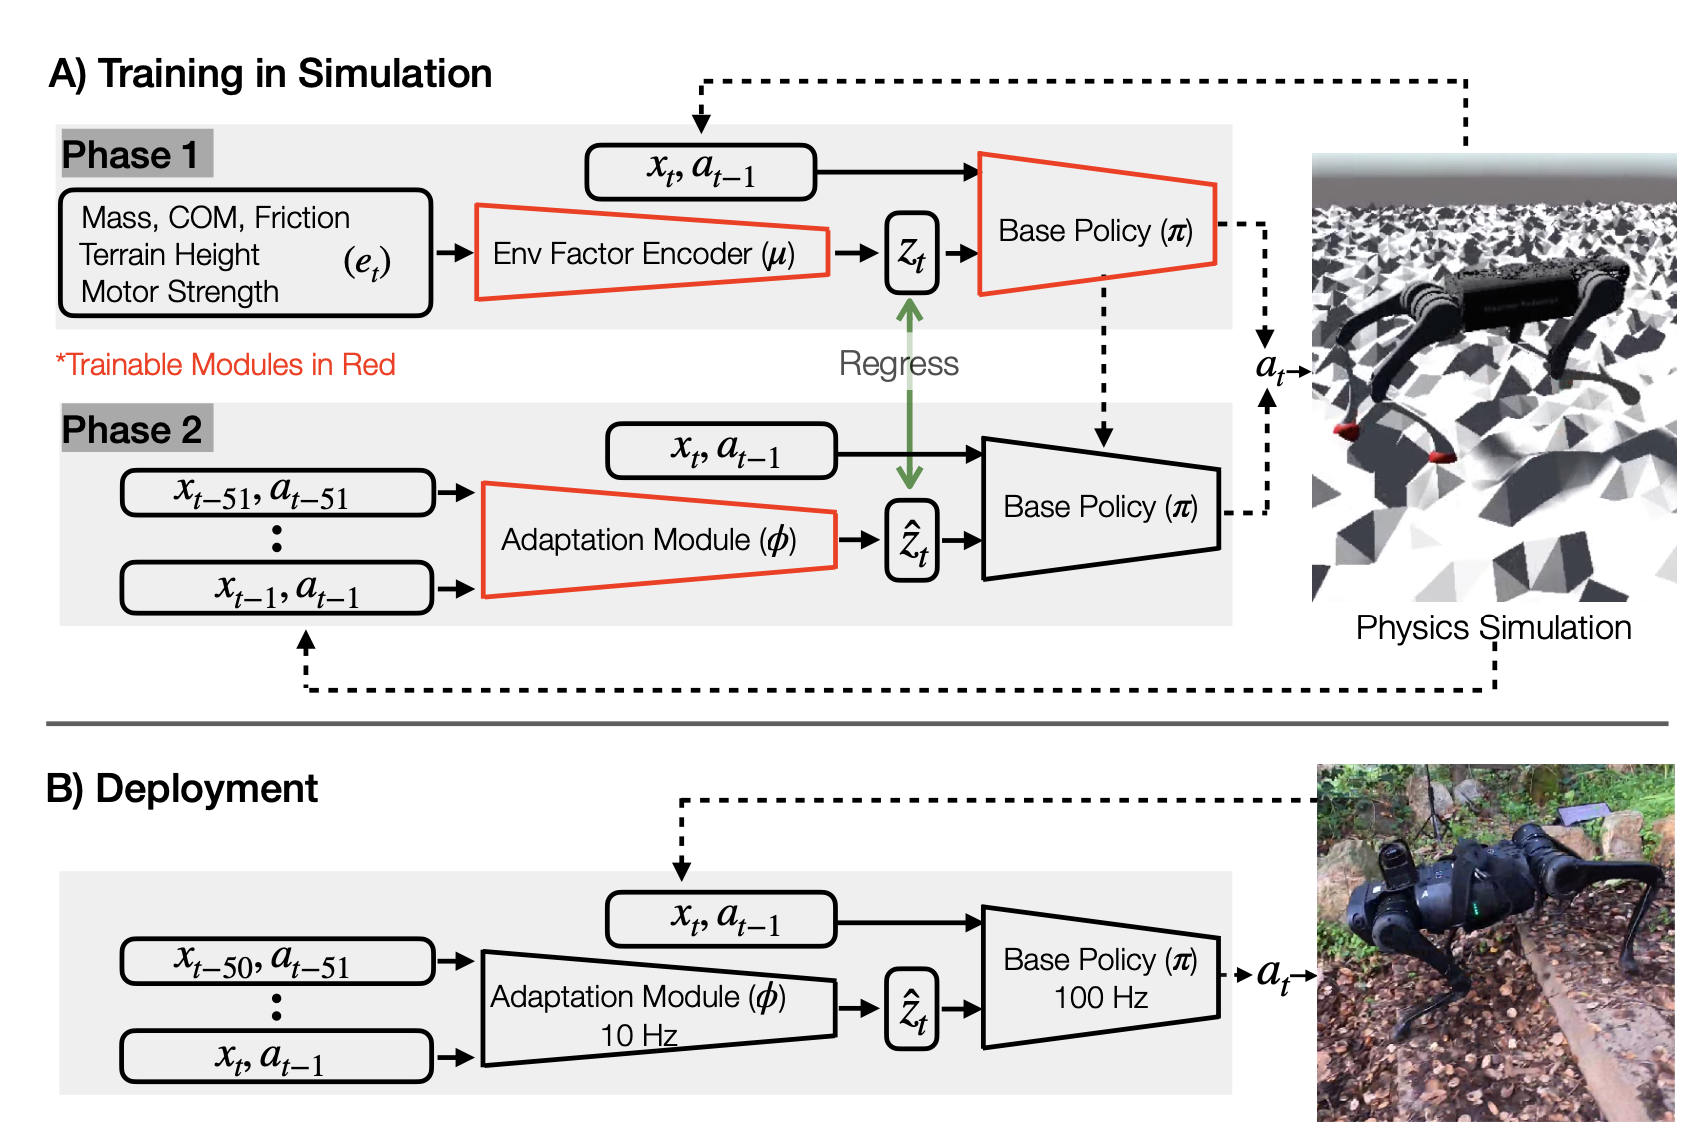
\includegraphics[scale=0.25]{../images/rma.png}

\end{frame}

\begin{frame}
  
  \frametitle{sample efficiency}

  \begin{itemize}
    \item intuitive unit {\bf one Montezuma experiment}
    \item 128M samples runs {\bf 65hours}
    \item eats less than {\bf 4G memory}
    \item fits {\bf 3 experiments} into single GPU (12G)
  \end{itemize}

  \bigskip

  \begin{itemize}
    \item RND \footnote{\href{https://arxiv.org/pdf/1810.12894.pdf}{Burda et al. 2018}} $4.5*10^9$ samples, score 8152 on MR
    \item Never give up \footnote{\href{https://arxiv.org/pdf/2002.06038.pdf}{Badia et al. 2020}} $3.5*10^{10}$ samples, score 10 000 on MR
    \item SND $1.28*10^8$ score 10 000 on MR 
  \end{itemize}

  NGU on my machine means {\bf 740 days} !!!
\end{frame}


\begin{frame}
  
  \frametitle{misleading papers - Curiosity-driven Exploration by Self-supervised Prediction \footnote{\href{https://arxiv.org/abs/1705.05363}{Pathak et al. 2017}}}
  
  \begin{itemize}
    \item not working on REAL hard exploration problems
    \item Super Mario is special case - moving forward is close to optimal policy
    \item inverse ICM model - why they didn't shown accuracy (my results arround 40\% !!! even given policy)
    \item how predicted state looks ?
  \end{itemize}

  \centering
  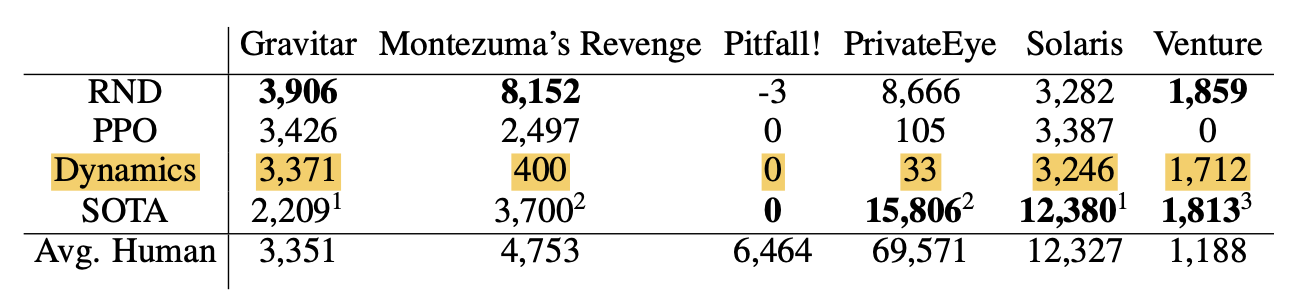
\includegraphics[scale=0.25]{../papers_captions/icm_a.png}

\end{frame}



\begin{frame}
  
  \frametitle{misleading papers - Never give up \footnote{\href{https://arxiv.org/pdf/2002.06038.pdf}{Badia et al. 2020}}}
  nice looking score, but on cost of $3.5*10^{10}$ samples !!!
  
  \centering
  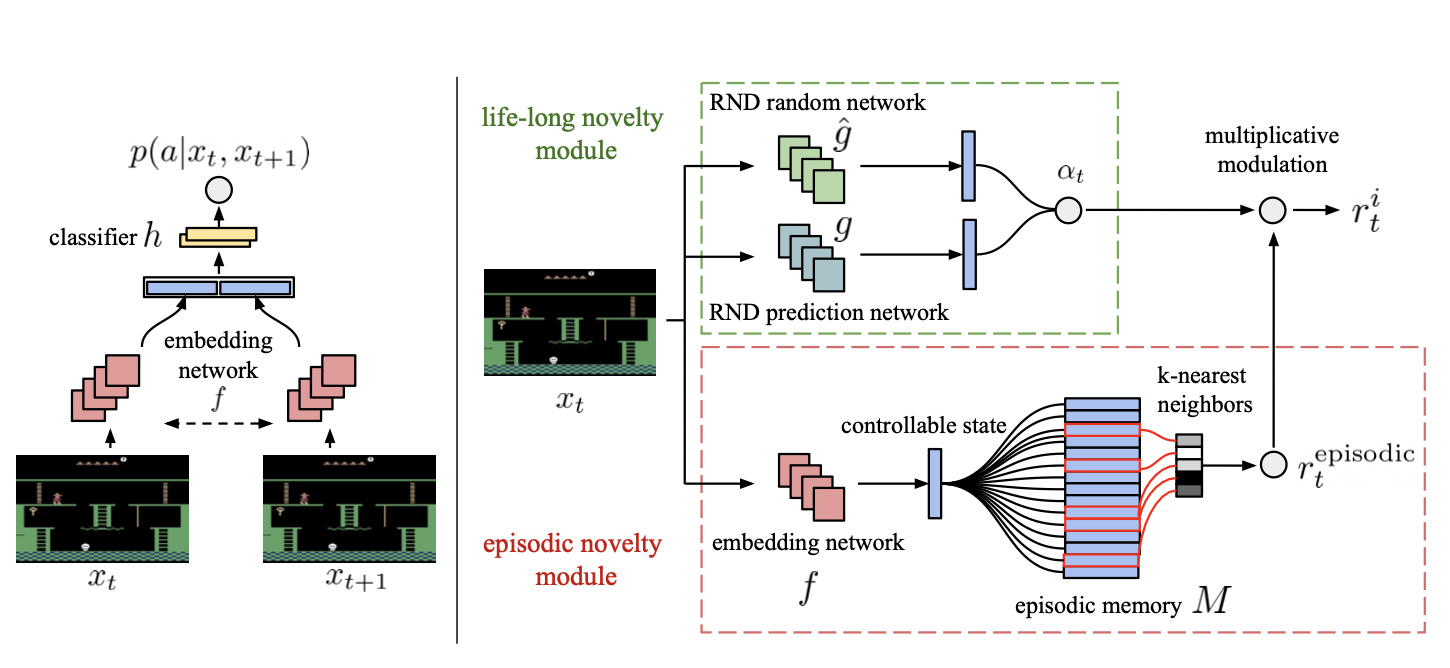
\includegraphics[scale=0.25]{../papers_captions/ngu_block.png}

  \centering
  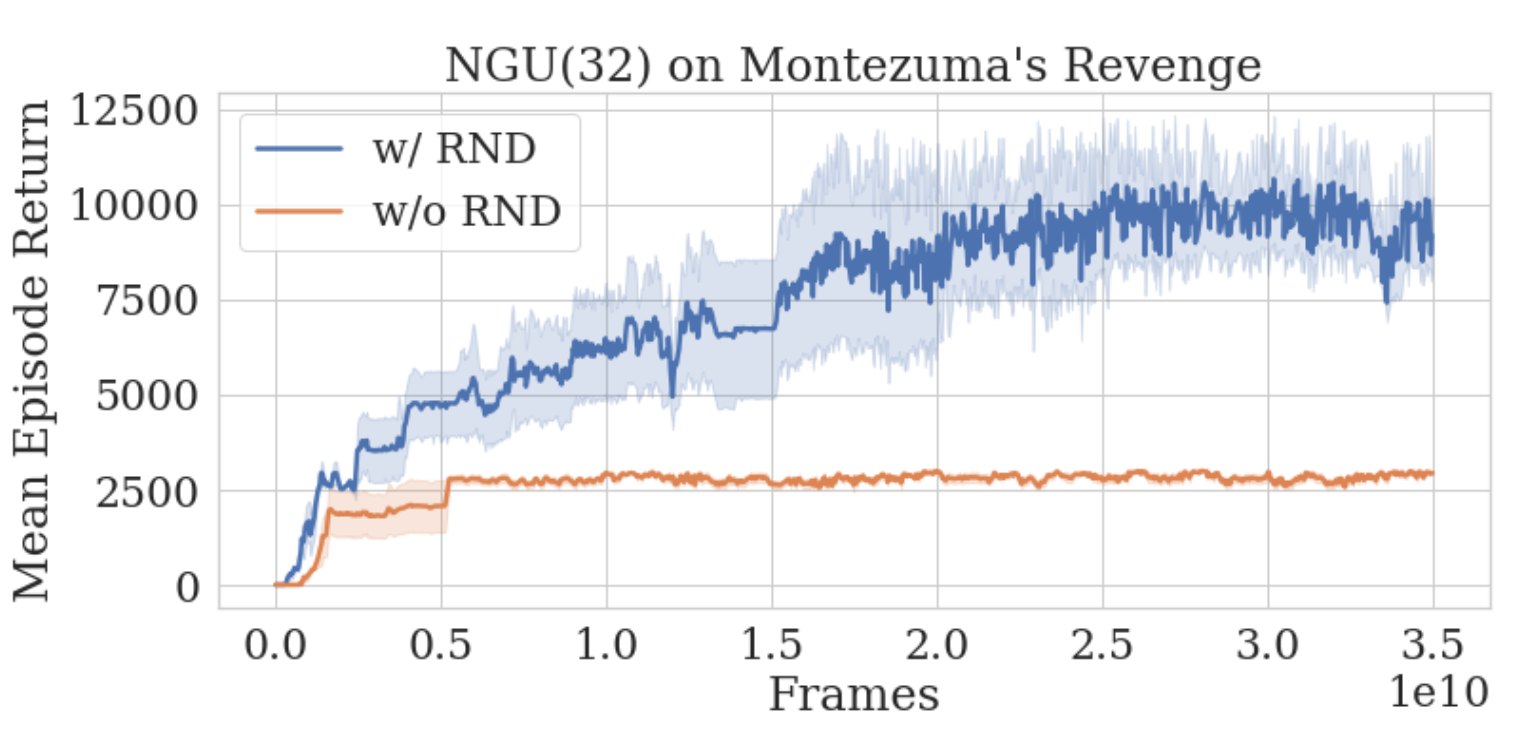
\includegraphics[scale=0.25]{../papers_captions/ngu_result.png}

\end{frame}



\begin{frame}
  
  \frametitle{other misleadings}

  \centering
  {\bf avoiding comparing with SOTA or common benchmarks results} :
  Episodic Curiosity Through Reachability, Savinov, 2019 
  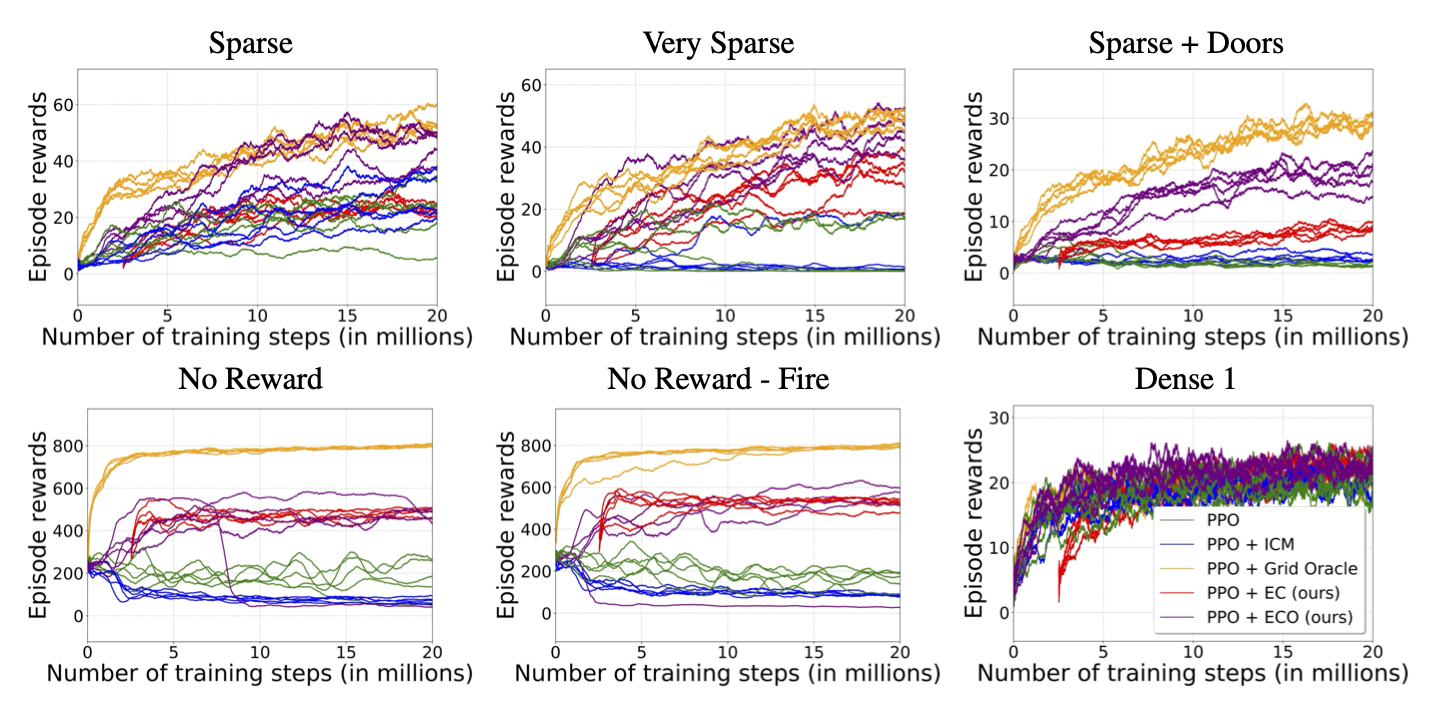
\includegraphics[scale=0.25]{../papers_captions/ecr.png}
  \bigskip

  many other :

  \begin{itemize}
    \item simple gridworld or toy environment experiments
    \item providing key prior information (e.g. possition)
    \item selecting only "good" results
  \end{itemize}

\end{frame}




\begin{frame}
  
  \frametitle{my current research}

    \begin{itemize}
      \item siamese network distillation - reached SOTA score with 1/100 samples
      \item symmetry driven generalisation, Noether's theorem in RL
    \end{itemize}

\end{frame}

\begin{frame}
  
  \frametitle{siamese network distillation}

  \centering
  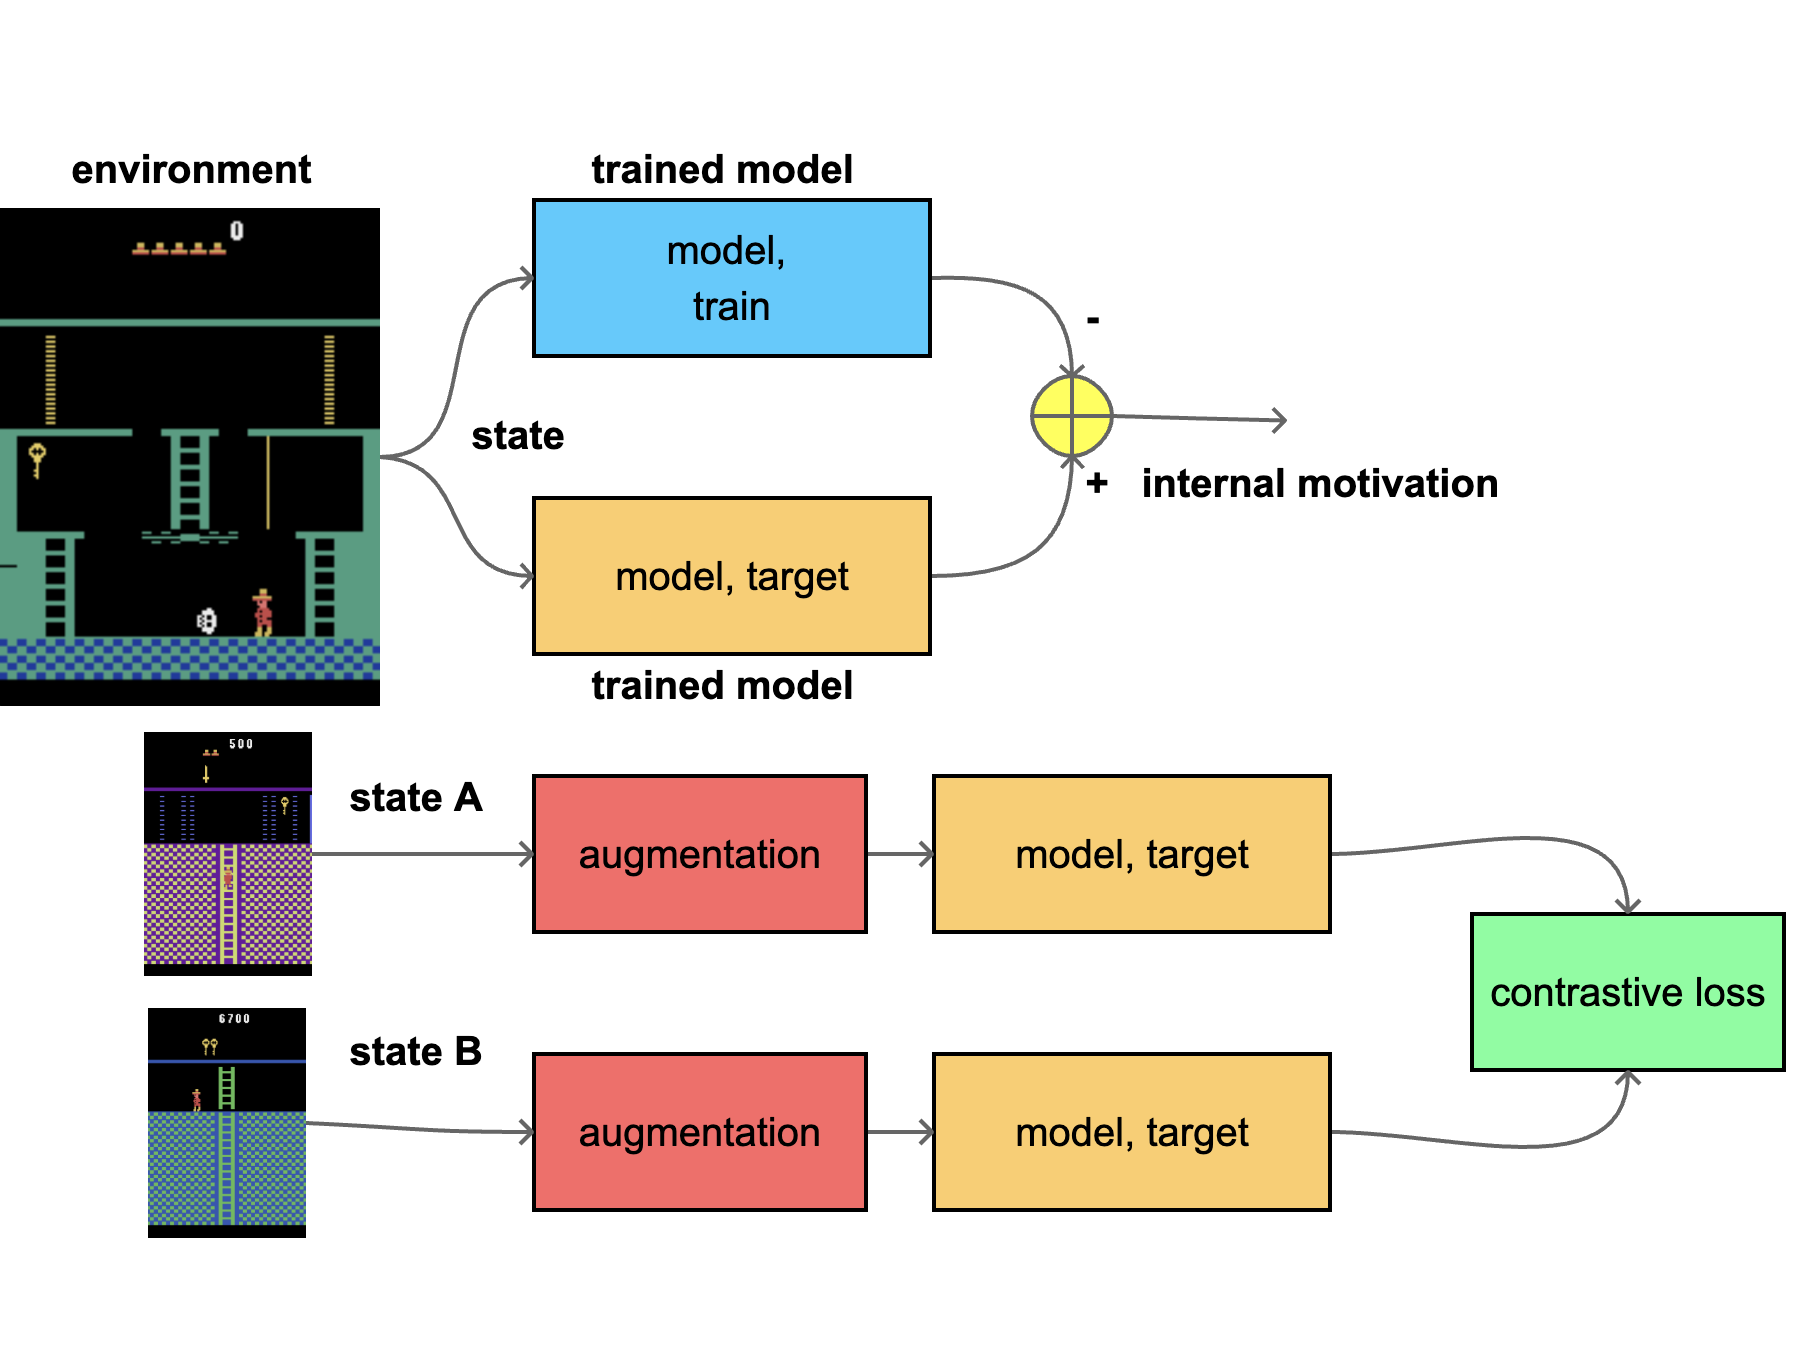
\includegraphics[scale=0.07]{../diagrams/rnd/rndsiamdetail.png}
  \bigskip
  \begin{columns}

    \begin{column}{0.5\textwidth}
      \centering
      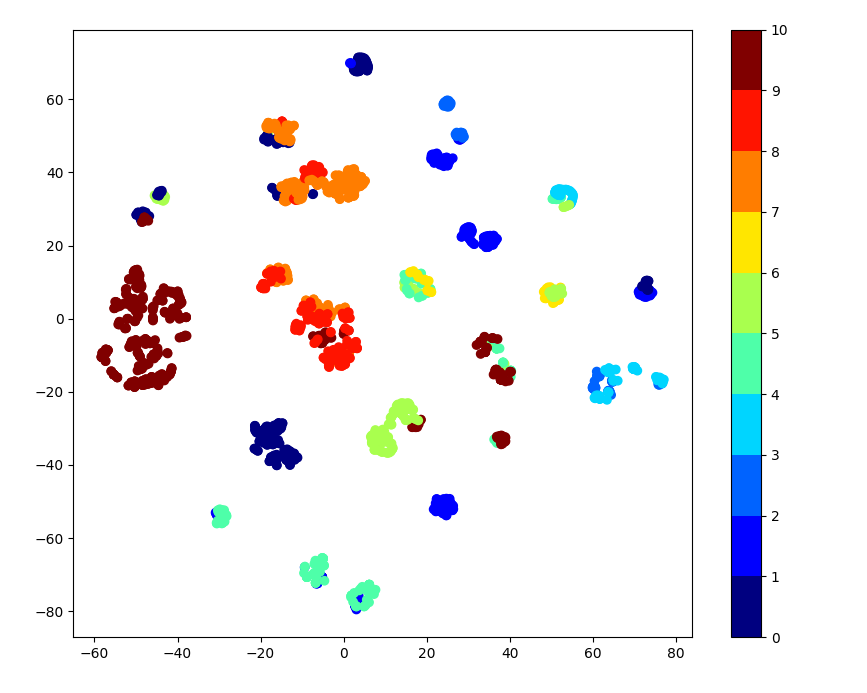
\includegraphics[scale=0.2]{../images/rnd_features.png}
    \end{column}

    \begin{column}{0.5\textwidth}
      \centering
      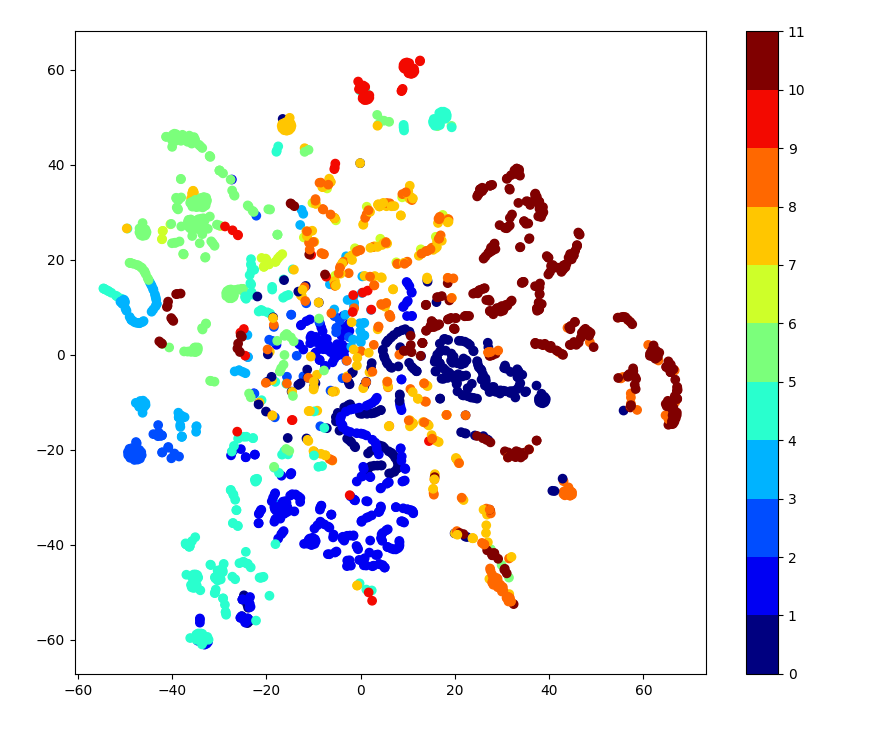
\includegraphics[scale=0.2]{../images/snd_features.png}
    \end{column}
  
  \end{columns}

\end{frame}

\begin{frame}
  
  \frametitle{symmetry driven generalisation \footnote{\href{https://geometricdeeplearning.com/lectures/}{Bronstein et al. 2021} Geometric deep learning - some trivial hand-crafted symmetries} }

  \centering
  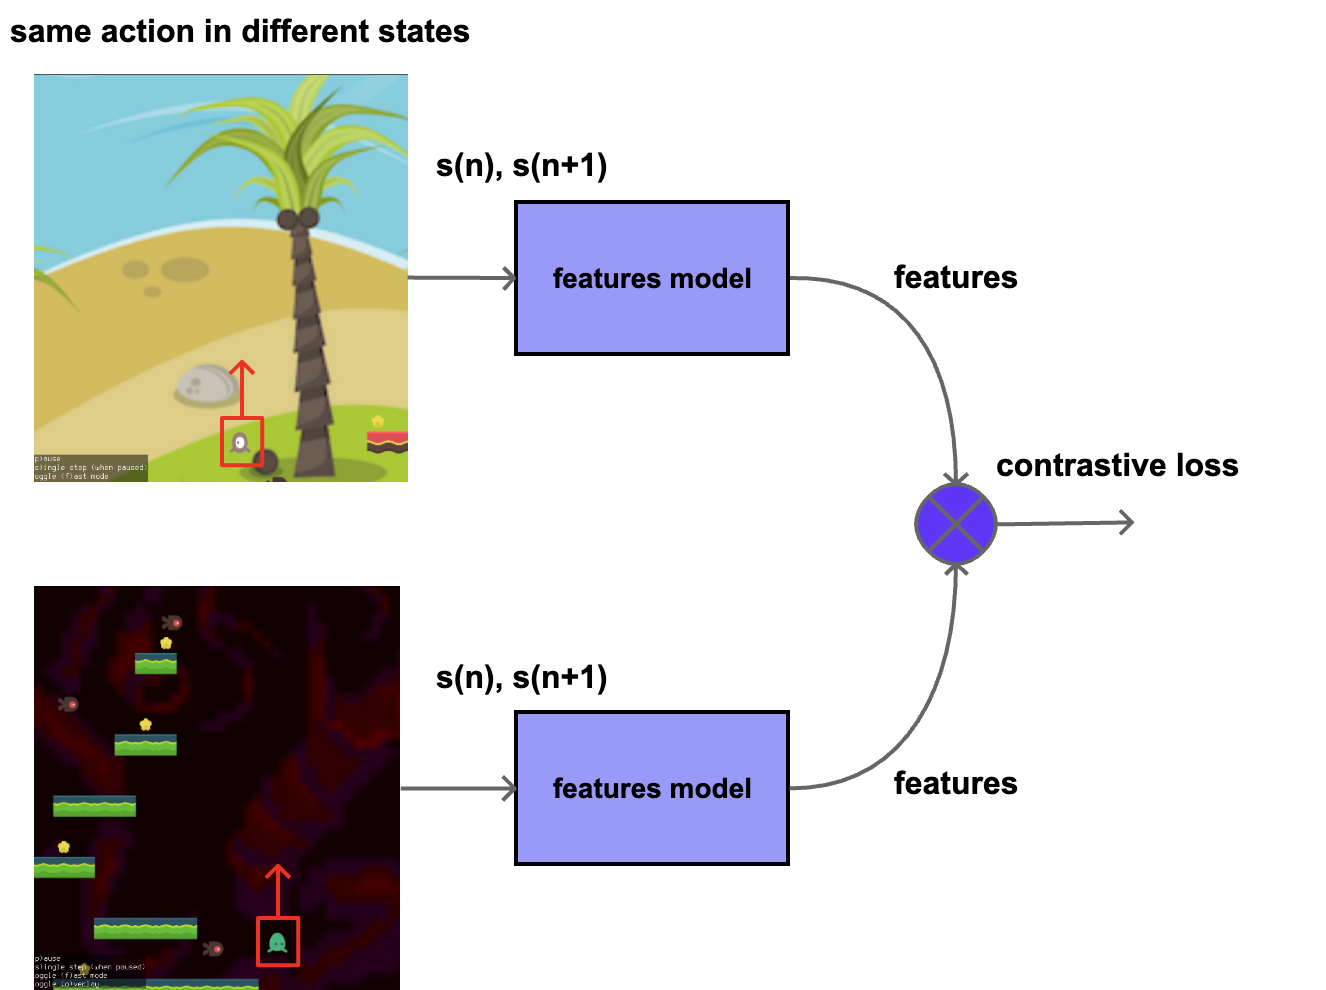
\includegraphics[scale=0.15]{../diagrams/symmetry/basic.png}

  \begin{align*}
    \forall (s_{n},s_{n+1} \vert a) : f \Big( s_{n}, s_{n+1}; \theta \Big) = const_a \footnotemark
  \end{align*} 
  \footnotetext{avoid trivial collapse}


   
\end{frame}


\begin{frame}
  
  \frametitle{recommended sources}

  \begin{itemize}
    \item book : Maxim Lapan, 2020, Deep Reinforcement Learning Hands-On second edition
    \item book : Enes Bilgin, 2020, Mastering Reinforcement Learning with Python
    \item youtuber : Yannic Kilcher, \href{https://www.youtube.com/c/YannicKilcher/videos}{link}
    \item youtuber : Two Minute Papers, \href{https://www.youtube.com/c/KárolyZsolnai/videos}{link}
    \item web : Paper With Code, \href{https://paperswithcode.com/methods/category/policy-gradient-methods}{link}
    \item web : Intellabs, \href{https://intellabs.github.io/coach/components/agents/index.html}{link}
  \end{itemize}
    
\end{frame}


\begin{frame}
  
  \frametitle{Q\&A}

  \begin{columns}

    \begin{column}{0.5\textwidth}
      \centering{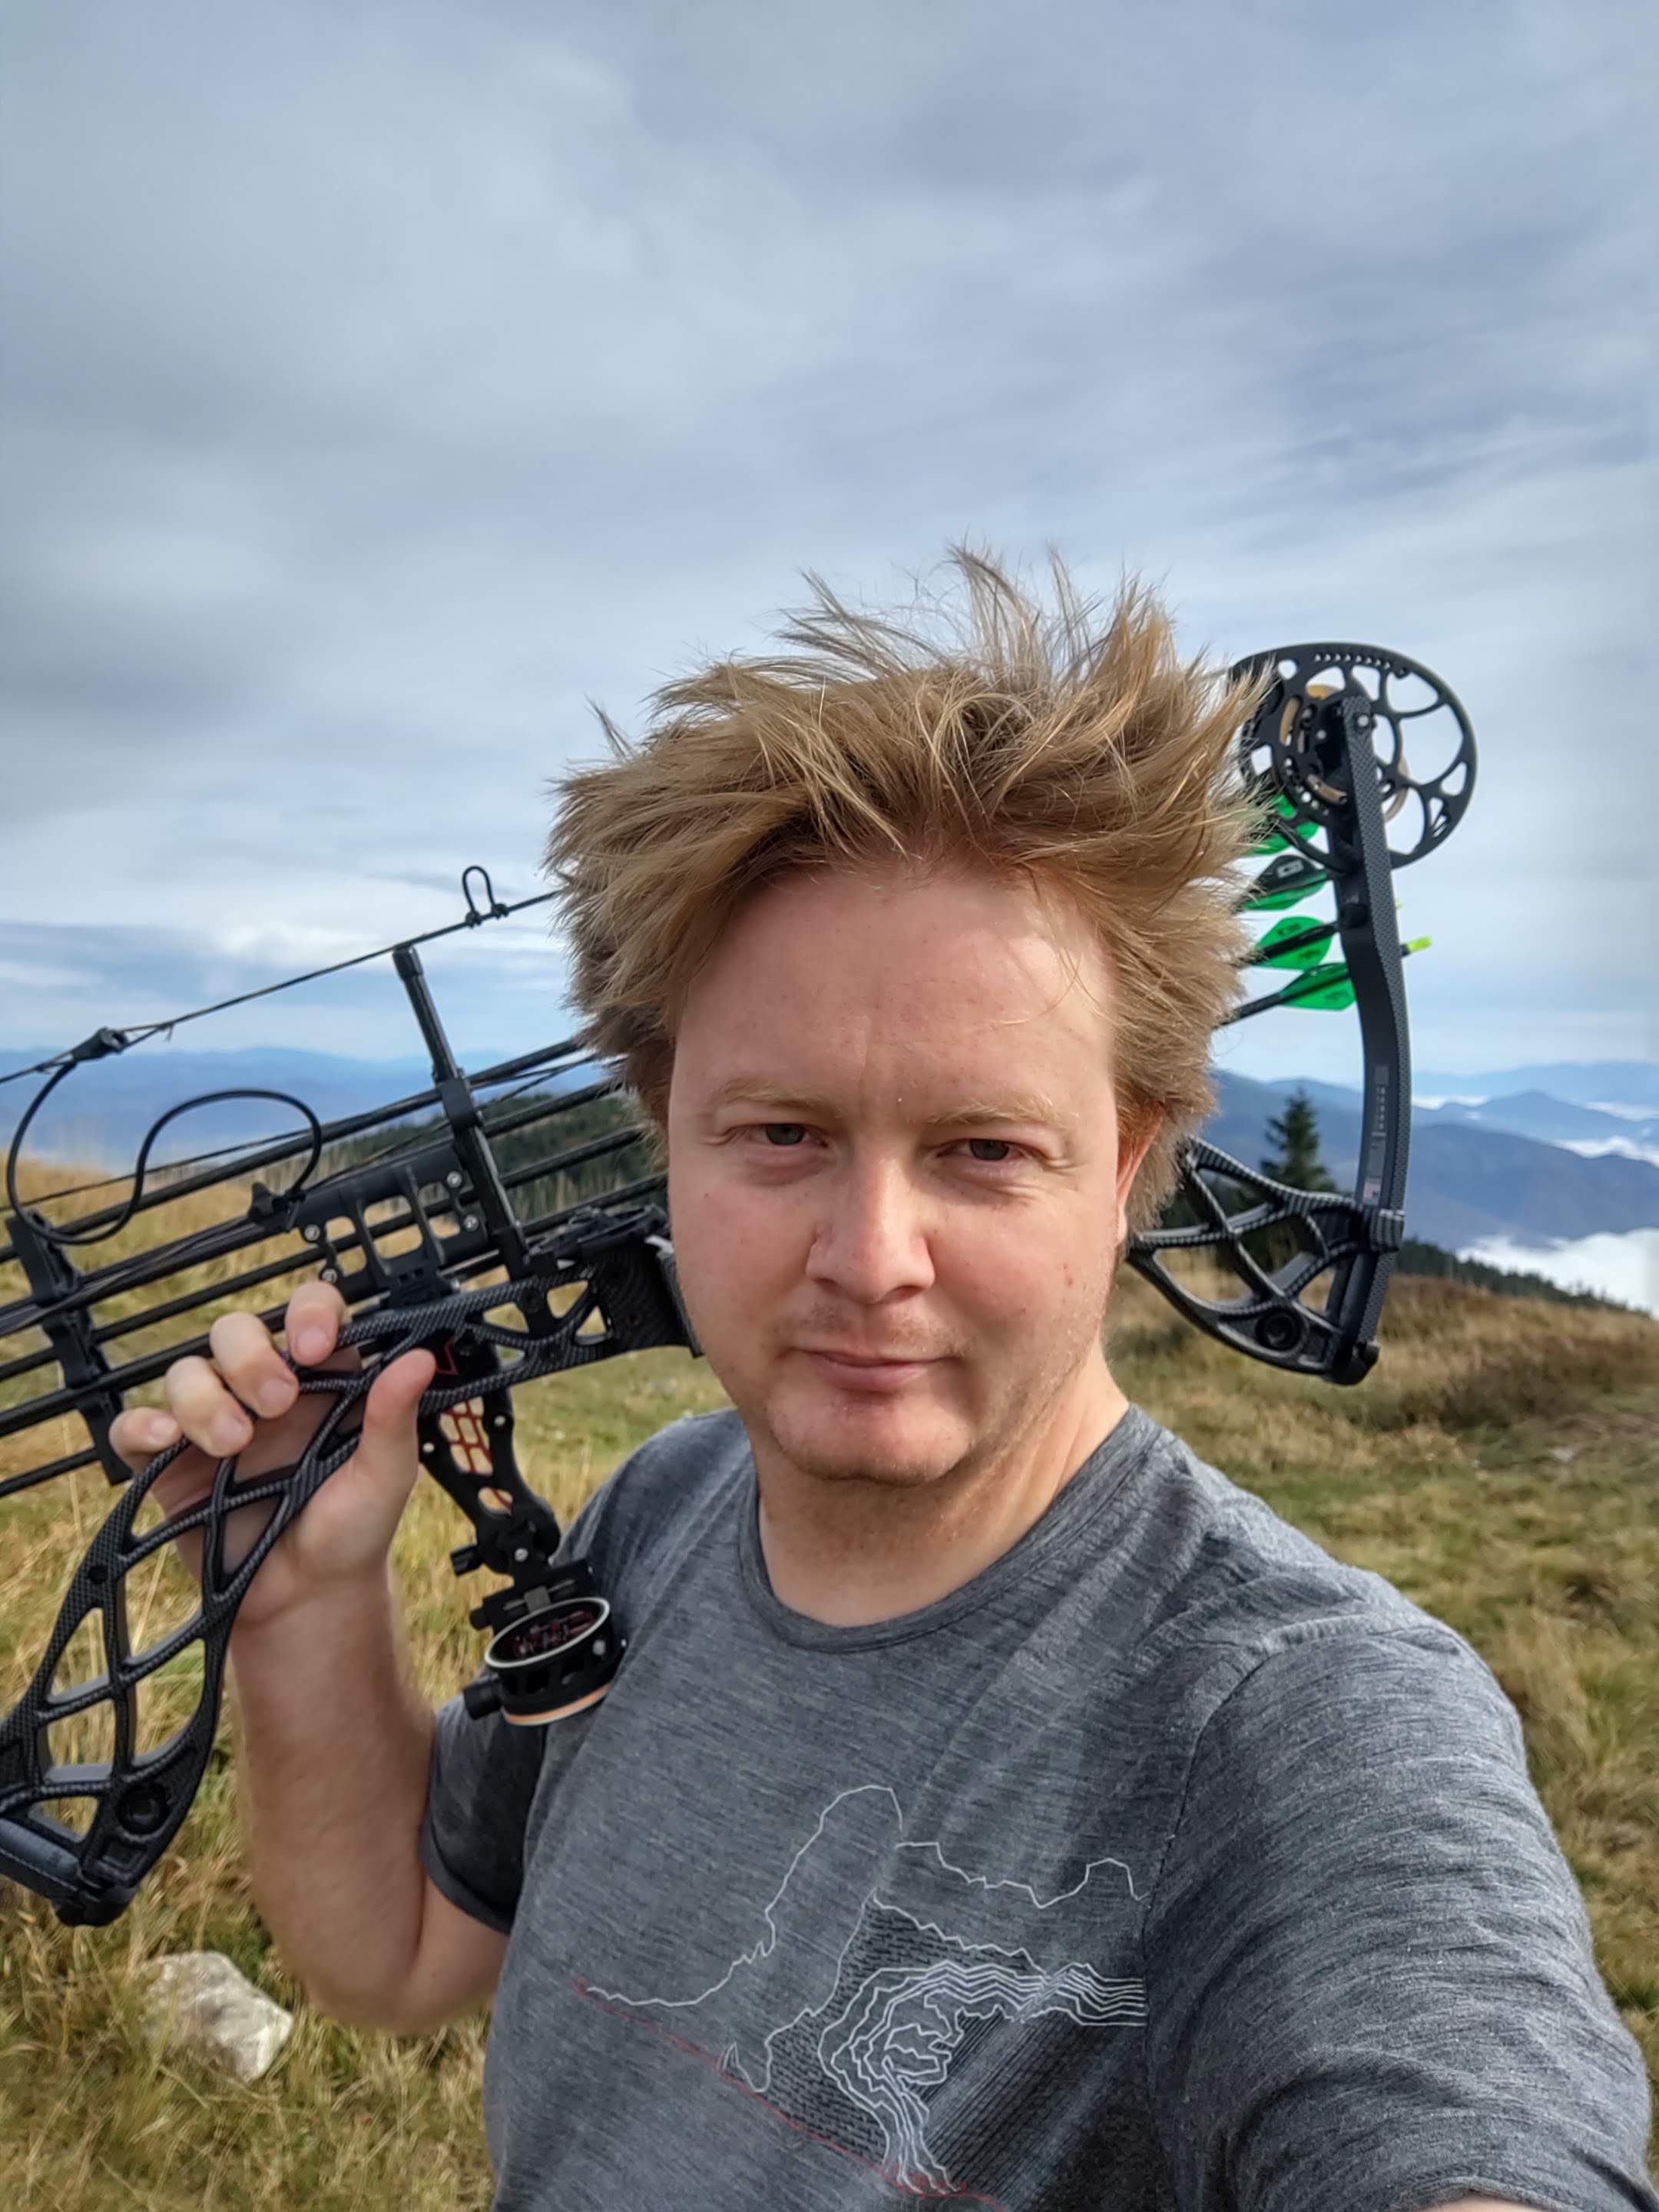
\includegraphics[scale=0.08]{../images/me3.jpg}}
    \end{column}

    \begin{column}{0.5\textwidth}
      \begin{itemize}
        \item \url{https://github.com/michalnand/}
        \item \url{michal.nand@gmail.com}
      \end{itemize}
    \end{column}

  \end{columns}

    
\end{frame}

\end{document}